\documentclass[11pt]{article}

\usepackage[a4paper,margin=1cm]{geometry}
\usepackage[utf8]{inputenc}
\usepackage[ngerman]{isodate}
\usepackage{gensymb}
\usepackage[x11names]{xcolor}
\usepackage{graphicx}
\usepackage{svg}
\usepackage{booktabs}% http://ctan.org/pkg/booktabs
\usepackage{makecell}
\usepackage{tabularx}
\usepackage{amsmath}
\usepackage{amssymb}
\usepackage{array}
\usepackage{wrapfig}
\usepackage{subcaption}
\usepackage{csquotes}
\usepackage{lscape}
\usepackage{afterpage}
\usepackage{listingsutf8}
\usepackage{geometry}
\usepackage{chngcntr}
\usepackage{multicol}
\usepackage{xcolor}
\usepackage{pifont}
\usepackage{outlines}
\usepackage{breqn}
\usepackage{textcomp}
\usepackage{bm}
\usepackage{enumitem}
\usepackage{mdframed}
\usepackage{scalerel}
\usepackage{stackengine}
\usepackage{mathtools}
\usepackage{hyperref}

% Code highlighting
\usepackage{minted}
\surroundwithmdframed{minted}

% Be able to caption equations and float them in place
\usepackage{float}
\usepackage{caption}

\newmdtheoremenv{theorem}{Theorem}

\DeclareCaptionType{equ}[Equation][List of Equations]

\counterwithin{figure}{section}

\AtBeginDocument{\counterwithin{lstlisting}{section}}

\geometry{a4paper, margin=1in}

\renewcommand*{\thead}[1]{\bfseries #1}
\newcommand{\code}[1]{\texttt{#1}}
\def\doubleunderline#1{\underline{\underline{#1}}}

\newcommand\equalhat{\mathrel{\stackon[1.5pt]{=}{\stretchto{%
				\scalerel*[\widthof{=}]{\wedge}{\rule{1ex}{3ex}}}{0.5ex}}}}

\newcommand\defeq{\mathrel{\overset{\makebox[0pt]{\mbox{\normalfont\tiny def}}}{=}}}

\newcolumntype{C}{>{\centering\arraybackslash}X}

\DeclarePairedDelimiter\abs{\lvert}{\rvert}
\DeclarePairedDelimiter\norm{\lVert}{\rVert}

\definecolor{lightgray}{rgb}{.9,.9,.9}
\definecolor{darkgray}{rgb}{.4,.4,.4}
\definecolor{purple}{rgb}{0.65, 0.12, 0.82}
\definecolor{darkgreen}{rgb}{0.05,0.56,0.06}
\definecolor{mauve}{rgb}{0.8863,0.5216,1}

\setcounter{tocdepth}{3}
\setcounter{secnumdepth}{3}

\graphicspath{{./img/}}
\svgpath{{svg/}}

\begin{document}

\title{Advanced Statistical Data Analyis HS19}
\author{Pascal Baumann\\pascal.baumann@stud.hslu.ch}
\maketitle

For errors or improvement raise an issue or make a pull request on the \href{https://github.com/KilnOfTheSecondFlame/mse_summaries}{github repository}.

\tableofcontents

\newpage

\section{Introduction}

In statistical analysis we talk about a response Variable $Y$, $i=1,2,3,....$, and a prediction variable $x_i^{(1)}, x_i^{(2)}, x_i^{(3)}, ..., x_i^{(p)}$. And we'd like to make a prediction like

\begin{equation*}
    y_i \approx f(x_i^{(1)}, x_i^{(2)}, x_i^{(3)}, ..., x_i^{(p)})
\end{equation*}

The problem is that the function $f$ is unknown. We can simplify and try to fit a linear model

\begin{equation*}
    y_i \approx \beta_0 + \beta_1\cdot x_i^{(1)} + \beta_2\cdot x_i^{(2)} + \cdots + \beta_p\cdot x_i^{(p)}
\end{equation*}

\subsubsection{Example}

$y \approx \beta_0 + \beta_1 x^{(1)} + \beta_2 log(x^{(2)})$ is linear in $\beta_0, \beta_1, \beta_2$, but $y \approx \beta_0 + \beta_1 (x^{(2)})^{\beta_2}$ is \underline{not} linear in $\beta_0, \beta_1, \beta_2$


\subsection{Linear Regression Model}
\begin{equation*}
    Y_i = \beta_0 + \beta_1\cdot x_i^{(1)} + \beta_2\cdot x_i^{(2)} + \cdots + \beta_p\cdot x_i^{(p)} + E_i
\end{equation*}
$E_i$ \: random variable $\sim \mathcal{N}(0, \sigma ^2)$ (where $\sim$ means stochastically independent). The most convenient assumptions are that these random variables $E_i$ are:

\begin{itemize}
	\item are (stochastically) independent
	\item have expectation zero and a constant variance $\sigma^2$ (as a function of $i$)
	\item are normally distributed (also called the Gaussian distribution)
\end{itemize}

\noindent
\begin{theorem}
	Linear Regression Model $\underline{Y} = \textbf{X} \underline{\beta} + \underline{E}\text{ with } \underline{E} \sim \mathcal{N}\langle \underline{0},\sigma^2\textbf{I}\rangle$
\end{theorem}

\vspace{1em}
\noindent
To build our model it's advisable to use the unifying class of linear models

\vspace{1em}
\begin{tabular}{l l}
	\hline
	Response & Model \\
	\hline
	Continuous (with constant variance) & Multiple linear regression model \\
	Zero/one variate & Logistic regression model \\
	Counts & Loglinear model \\
	Continuous (with constant coefficient of variation) & Gamma regression model \\
	Censored survival times & Accelerated Failure Time Models,\\
	& Proportional hazard model \\
	\hline
\end{tabular}

\subsubsection{Least squares}
From the example dataset MTCars
\begin{equation*}
    \sum_{i=1}^n ( \underbrace{lMPG_i - (\beta_0 + \beta_1 lDisp_i + \cdots \beta_m wGear_i)}_{\text{Residual }r_i (\equalhat,'\approx')})^2 = min_{\beta_0, \beta_1, ..., \beta_m }
\end{equation*}
gives the estimated coefficients $\Rightarrow \beta_0, \beta_1, ..., \beta_m $

\vspace{1em}

\noindent
The least squares method expects the error term $E_i$ to be normally distributed. If that is not the case the model is not ideal.

\subsubsection{Maximum Likelihood Principle}
We expect the error $\epsilon_i = \underline{y} - \textbf{X}\underline{\beta}$ to be normally distributed, hence the likelihood function becomes:
\begin{equ}[H]
	\begin{equation*}
		\Phi_{\mu, \sigma}(x) = \frac{1}{\sqrt{2\pi}\sigma}e^{\frac{(x-\mu)^2}{2\sigma^2}}
	\end{equation*}
	\caption{Normal distribution model}
\end{equ}

\begin{equ}[H]
	\begin{equation*}
		L\langle \underline{\beta},\sigma | \underline{y}, \textbf{X}\rangle = \frac{1}{(2\pi\sigma^2)^{n/2}}e^{\left\langle-\frac{1}{2\sigma^2}(\underline{y}-\textbf{X}\underline{\beta})^T(\underline{y}-\textbf{X}\underline{\beta})\right\rangle}
	\end{equation*}
	\caption{Maximum Likelihood Function $L$ for a Linear Regression model}
\end{equ}

Miminising the maximum likelihood function is the same as minimising the log likelihood function:

\begin{equ}[H]
	\begin{equation*}
		\text{log}(L\langle \underline{\beta},\sigma | \underline{y}, \textbf{X}\rangle) = -\frac{n}{2}\text{log}\langle2\pi\rangle -\frac{n}{2}\text{log}\langle\sigma^2\rangle -\frac{1}{2\sigma^2}(\underline{y}-\textbf{X}\underline{\beta})^T(\underline{y}-\textbf{X}\underline{\beta})
	\end{equation*}
	\caption{Log Likelihood Function}
\end{equ}

The partial derivative of this function for the parameters $\underline{\beta}$ equal to zero, will give us the best estimation for $\underline{\beta}$.


\subsubsection{Result from statistical inference}

\begin{equation*}
    \underline{\widehat{\beta}} \sim \mathcal{N}(\underline{\beta},\sum_\beta), \widehat{\sqrt{Var(\tilde{\beta_n})}} = se(\tilde{\beta_n})
\end{equation*}
\noindent
Reduced model: $r_i^{(r)}$
\\
Full model: $r_i^{(f)}$

\begin{equation*}
    \frac{\frac{1}{q}(\sum{(r_i^{(r)}})^2 - (r_i^{(f)})^2)}{\frac{1}{n-p}\sum{(r_i^{(f)})^2}} \sim F_{n-p,q}
\end{equation*}

With this we can check if the reduced model is similar to the full model.

\subsection{Akaike's Information Criterion (AIC)}
A sensible variable selection criterion must combine measures of \textbf{model accuracy} and \textbf{model complexity}. But these two types of measurement are conflicting as additional explanatory variables always lead to a higher model accuracy but also to higher model complexity. The most popular variant of such a criterion is the \textbf{Akaike Information Criterion} which weighs goodness-of-fit against the complexity of the model:
\begin{align*}
	AIC &= -2 (maximised\ log\ likelihood) + 2 (number\ of\ estimated\ parameters)\\
	&= n\ \text{log}\left\langle \frac{1}{n}\sum_{i=1}^{n}R_i^2\right\rangle + 2 p^\diamond + \text{constant}
\end{align*}

Where $p^\diamond$ is the number of all estimated parameters, including $\widehat{\sigma}$

\subsection{Tukey's First Aid Transformations}
Neither the explanatory variables nor the response variable do have to be linear. If there is no guidance for transformation of the variables based on subject matter theory, a good start are the following recommendations which are based on experiences of statistical data analysis and often lead to simple and plausible models, and are called \textbf{Tukey's First Aid Transformations}
\begin{itemize}[label=-]
	\item use a logarithm transformation for concentrations and amounts, in general for continuous variables that can only have positive values
	\item use the square root or a logarithm transformation for count data
	\item use the so-called logit transformation $\tilde{x} = \log\left\langle \frac{x+0.005}{1.01-x} \right\rangle$ for counted fractions or shares
\end{itemize}

\section{Review of Linear Regression Modelling}

\subsection{Residuals}
If $\underline{\widehat{y}} = \textbf{X}\underline{\widehat{\beta}} = \textbf{X} (\textbf{X}^T \textbf{X})^{-1} \textbf{X}^T \underline{Y}$
\begin{equation*}
	\textbf{H} = \textbf{X} (\textbf{X}^T \textbf{X})^{-1} \textbf{X}^T
\end{equation*}

\noindent
Where $\textbf{H}$ is called the projection matrix. And the residual vector can be calculated as follows:

\begin{equation*}
	\underline{R} = \underline{Y} - \textbf{X} \underline{\widehat{\beta}} = \underline{Y} - \textbf{H} \underline{Y} = (\textbf{I} - \textbf{H}) \underline{Y}
\end{equation*}

\noindent
With the expectation

\begin{equation*}
	\mathbb{E}\langle\underline{R} \rangle = \mathbb{E}\langle\underline{Y} - \textbf{X} \underline{\widehat{\beta}} \rangle = \textbf{X} \underline{\widehat{\beta}} - \textbf{X} \underline{\widehat{\beta}} = \underline{0}
\end{equation*}

\noindent
and variance
\begin{equation*}
	\text{var}\langle \underline{R} \rangle = \text{var}\langle (\textbf{I} - \textbf{H}) \underline{Y} \rangle = \sigma^2 (\textbf{I} - \textbf{H})
\end{equation*}

\noindent
Thus the \textbf{scaled residuals} $\breve{R}_i$ have the same marginal distribution as the errors $E_i$ but are still correlated.
\begin{equation*}
	\breve{R}_i = \frac{R_i}{\sqrt{1-H_{ii}}}, i=1..n
\end{equation*}

\noindent
Often the so-called \textbf{standardised residuals} $\tilde{R}_i$ are used in residual analysis.

\begin{equation*}
	\tilde{R}_i = \frac{R_i}{\sqrt{\widehat{\sigma}^2(1-H_{ii})}}, i=1..n
\end{equation*}

\subsection{Model Adequacy Checking}
\subsubsection{Diagnostic Plots}
Are used to get information about the data and the used model

\vspace{1em}
\noindent
\begin{tabularx}{\textwidth}{l X X}
	\hline
	\textbf{Name} & \textbf{Description} & \textbf{Property}\\
	\hline
	\textbf{Tukey-Ascombe Plot} & Residual plot which plots the residuals against the fitted values & detect non-constant expectation of the errors\\
	\textbf{Scale-Location Plot} & The square-root of the absolute values of the standardised residuals plotted against the fitted values & detect non-constant variance of the errors\\
	\textbf{Normal Q-Q Plot} & Ordered standardised residuals plotted against their expected values under the assumption of normality & detect non-normality of the errors\\
	\textbf{Residuals against Time} & & detect stochastic dependency\\
	\textbf{and/or space variables} & & in the errors\\
	& & \\
	\textbf{Sensitivity Plot} & Standardised residuals plotted against the leverage overlaid by Cook's distance contours & detect too influential observations in the data\\
\end{tabularx}

\subsection{Leverage}
The leverage asks how much the estimation for $\beta$ changes when we remove a certain observation.
If the Cook's distance of $d_i$ is larger than one, the $i$th observation has too much influence. If the leverage is greater than $0.2$ the observation could have too much leverage, with $0.5$ the leverage is too big.

\subsubsection{Multicollinearity}
To detect collinearity, one can examine the correlation matrix of the predictors, which will reveal large pairwise collinearities. Alternatively, one can consult the \textbf{Variance Inflation Factor}

\begin{equation*}
	var\langle \widehat{\beta}_k \rangle = \sigma^2 \frac{1}{1-R_k^2}\frac{1}{\sum_{i=1}^k (x_i^{(k)} - \bar{x}_k)^2}
\end{equation*}

The middle term $\text{VIF}_k = \frac{1}{1-R_k^2}$ is the factor with which the variance of the estimated parameter $\widehat{\beta}_k$ is inflated when multicollinearity exists.

\paragraph{Guideline} If $\text{VIF}_k$ is larger than 5-10 for any variable, then the multicollinearity is of a dangerous size and need to be addressed.

\subsection{Back to the Cars dataset}

\begin{align*}
	\text{MPG}_i &= e^{\beta_0 + log(\text{WT}_i ^ {\beta_1)} + log(\text{HP}_i ^ {\beta_2)} + \text{E}_i}\\
	\text{gpm}_i &= e^{- \beta_0 - log(\text{WT}_i ^ {\beta_1)} - log(\text{HP}_i ^ {\beta_2)} - \text{E}_i}\\
	&= e^{-\beta_0}\cdot \text{WT}_i^{-\beta_1} \cdot \text{HP}_i^{-\beta_2} \cdot e^{- \text{E}_i}\\
	&= e^{-\beta_0}\cdot \text{WT}_i^{-\beta_1\beta_2} \cdot \frac{\text{HP}_i}{\text{WT}_i}^{-\beta_2} \cdot e^{- \text{E}_i}
\end{align*}

\subsection{Categorical Predictors}
Imagine a predictor variable with two levels A and B, to be able to include this categorical variable a indicator variable is set up:
\begin{equation*}
	x_i = \left\{ \begin{matrix}
		0 & \text{level A}\\
		1 & \text{level B}
	\end{matrix}
	\right.
\end{equation*}
\noindent
With this we can model the response as follows
\begin{equation*}
	Y_i = \beta_0 + \beta_i x_i + \beta_1 x_1 + \cdots + E_i
\end{equation*}
\noindent
To interpret the model
\begin{align*}
	\text{level A} \rightarrow x_i &= 0 \text{ hence } Y_i = \beta_0 + \beta_1 x_1 + \cdots + E_i\\
	\text{level B} \rightarrow x_i &= 1 \text{ hence } Y_i = (\beta_0 + \beta_i) + \beta_1 x_1 + \cdots + E_i
\end{align*}

\subsection{Prediction Error Sum of Squares (PRESS)}

In predictive modelling, the models are often assessed by the \textbf{leave-one-out method}:
\begin{enumerate}
	\item Select an observation $y_i$
	\item Fit the regression model to the remaining $n-1$ observations
	\item Predict the withheld observation $y_i$ with the model
\end{enumerate}
\noindent
Denoting this withheld observation $\widehat{y}_i$, the prediction error for the observation $i$ becomes $r_i = y_i -\widehat{y}_i$. And the \textbf{prediction error sum of squares} is thus defined as the sum of squares for the $n$ prediction errors

\begin{equation*}
	\text{PRESS} = \sum_{i=1}^{n} r_i^2 = \sum_{i=1}^{n} (y_i -\widehat{y}_i)^2
\end{equation*}

\section{Some Advanced Topics in Linear Regression Modelling}
\subsection{Some points to the preceding topics}
\begin{itemize}
	\item We always have to specify the Error term and it's distribution in a linear regression model
	\item A model acquired with the least squares method implicitly assumes a Normal distribution for the error terms
	\item \textbf{vif} - Variance Inflation Factor - Detects and measures multi-collinearity; if $\text{vif} > 10$ a collinearity or multi-collinearity problem exists
\end{itemize}

\subsection{Weighted Least Squares}
Sometimes the variance is not constant, we can attribute for that if we replace the identity matrix in the model

\begin{equation*}
	\textbf{Y} = \textbf{X}\beta + \text{E}\quad\text{ with }\text{E}\sim\mathcal{N}\langle 0, \sigma^2 \textbf{I}\rangle
\end{equation*}

\noindent
With a weight matrix

\begin{equation*}
	\textbf{W} = \textbf{I}\cdot \begin{bmatrix}
		\frac{1}{w_1}\\
		\frac{1}{w_2}\\
		\frac{1}{w_3}\\
		\vdots\\
		\frac{1}{w_n}
	\end{bmatrix}
\end{equation*}

\noindent
When we apply the Maximum Likelihood principle, we get two normal equations

\begin{align*}
	\textbf{X}^T \textbf{W}\underline{R} &= \underline{0}\\
	\textbf{X}^T \textbf{W}(\underline{Y}-\textbf{X}\underline{\widehat{\beta}}) &= \underline{0}
\end{align*}

\noindent
If the matrix $\textbf{X}$ has a full rank and all weights $w_i$ are greater than zero, there is the unique and explicit solution
\begin{equation*}
	\underline{\widehat{\beta}} = (\textbf{X}^T\textbf{W}\textbf{X})^{-1}\textbf{X}^T\textbf{W}\underline{Y}	
\end{equation*}

\subsection{Robustness}
How robust an estimator is, can be investigated by two simple measures, the \textbf{influence function} and gross error sensitivity, and the \textbf{breakdown point}.
Both measures are based on the idea of studying the reaction of an estimator under the influence of gross errors, that is arbitrary included data.

\begin{itemize}[leftmargin=*, labelindent=4cm, labelsep=0.5cm]
	\item[\textbf{gross error sensitivity}] is based on the influence function and measures the \textbf{maximum effect of a single observation on the estimated value}
	\item[\textbf{breakdown point}] returns the minimum proportion of data that can be altered without causing completely unreliable estimates
\end{itemize}
\noindent
Hence an estimator with good robustness properties has a bounded sensitivity and a breakdown point of around 0.5.
\noindent
When we want to limit the influence of an outlier, we have to limit the influence of the residuals with smaller weights. This $\psi$-function must be bounded.

\begin{equation*}
	\psi(r_i) \defeq w_i \cdot r_i
\end{equation*}

\noindent
The weights can then be determined with $w_i = \frac{\psi\langle r_i \rangle}{r_i}$, this is an iterative process as the weights depend on the true parameter $\underline{\beta}$. An estimator with such implied weights is called a robust \textbf{regression M-estimator}.

\noindent
Unfortunately M-estimators cannot cope with contaminated leverage points, and it's also not possible to identify such leverage points with Leverage and Cook's distance.

\section{Binary Response}

Linear regression cannot adequately represent the data, in the case of binary responses we usually use the Logistic Regression model, which we can introduce as follows

\begin{theorem}
	The response $Y$ is binary with possible values 0 and 1. Its distribution is given by the probability that it takes the value 1: $ \pi = P\langle Y = 1 \rangle$. In other words, the response $Y$ is Bernoulli distributed with unknown parameter $\pi$. If we consider $Y_k$ the response variable, it is binomial distributed with known parameter $m_k$ and unknown parameter $\pi$.
\end{theorem}

If a simple linear model were applicable, we would expect to see a linear relationship between $\tilde{Y}_k$ and $x_k$ in the Anaesthesia example. However, when we plotted the data in a scatter plot, this was not the case. We found a non-linear relationship which looked like a distribution function $G\langle \cdot \rangle$. This suggests modelling $\pi$ by

\begin{equation*}
	\pi\langle x_k \rangle = G\langle \beta_0 + \beta_1 \cdot x_k \rangle
\end{equation*}

\noindent
or equivalently by
\begin{equation*}
	G^{-1}\langle\pi\langle x_k \rangle\rangle = \beta_0 + \beta_1 \cdot x_k
\end{equation*}

\subsection{Latent Variable}
This approach also has a simple theoretical justification. Suppose that each patient has an unobserved “attribute”, expressed as a random variable $T$, which describes the anaesthetic depth – the random variable is also called \textbf{latent variable}. The response $Y_i$ records whether $T$ is below a threshold $c (Y_i = 0)$ or above it $(Y_i = 1)$. The threshold is set so that the anaesthetic depth $T$ above the threshold is sufficient for the operation. Then, the function $G\langle \cdot \rangle$ is the distribution function of the standardized latent variable $T$.

\begin{equation*}
	T_i = \beta_0 + \beta_1 \cdot x_i + \tau\cdot T_i^0
\end{equation*}

\noindent
Where $T_i^0$ would be the normal distributed error.

\subsection{Distribution Function}
Popular choices for the distribution function $G$ depend on the model

\vspace{1em}
\noindent
\begin{minipage}{\textwidth}
	\renewcommand{\arraystretch}{1.5}
	\begin{tabularx}{\textwidth}{C C p{6cm}}
		\hline
		$G\langle \eta \rangle$& $G^{-1}\langle \pi \rangle$ & Name \\
		\hline
		$\frac{\text{exp}\langle \eta \rangle}{1 - \text{exp}\langle \eta \rangle}$& $\text{log}\langle \frac{\pi}{1-\pi} \rangle$ & logit model, logistic regression \\
		$\Phi\langle \eta \rangle$& $\Phi^{-1}\langle \pi \rangle$ & probit model \\
		$1-\text{exp}\langle -\text{exp}\langle \eta \rangle \rangle$& $\text{log}\langle -\text{log} \langle 1-\pi \rangle \rangle$ & complementary log-log model \\
		\hline
	\end{tabularx}
\end{minipage}

\vspace{1em}
\noindent
whereas the $G^{-1}\langle\cdot\rangle$ is called the \textbf{canonical link function}.

\vspace{1em}
\noindent
\begin{tabularx}{\linewidth}{l l X}
	\textbf{Distribution} & \textbf{Canonical Link Name} & \textbf{Link Function} $\textbf{X}\boldsymbol{\beta} = g(\mu)$\\
	\hline
	Normal & Identity & $\textbf{X}\boldsymbol{\beta} = \mu$\\
	Exponential & Negative Inverse & $\textbf{X}\boldsymbol{\beta} = -\mu^{-1}$\\
	Gamma & Negative Inverse & $\textbf{X}\boldsymbol{\beta} = -\mu^{-1}$\\
	Poisson & Log & $\textbf{X}\boldsymbol{\beta} = \log(\mu)$\\
	Categorical & Logit & $\textbf{X}\boldsymbol{\beta} = \log(\frac{\mu}{1-\mu})$\\
	Multinomial & Logit & $\textbf{X}\boldsymbol{\beta} = \log(\frac{\mu}{1-\mu})$
\end{tabularx}

\subsection{Summary}
The logistic regression model is determined by assuming that
\begin{enumerate}
	\item the response is independently and binomially distributed (which includes the Bernoulli distribution)
	\item the linear predictor, that is a linear combination of the explanatory variables
	\begin{equation*}
		\eta = \beta_0 + \beta_1 x_1 + ... + \beta_m x_m
	\end{equation*}
	is
	\item linked to the parameter of success $\pi$ using the logistic (distribution) function:
	\begin{equation*}
		\pi = G\langle\eta\rangle = \frac{\text{exp}\langle \eta \rangle}{1 - \text{exp}\langle \eta \rangle}
	\end{equation*}
\end{enumerate}

\section{Unifying Model}

It is worth summarising the components of both the logistic regression model and the classical multiple linear regression model.
Both models involve
\begin{itemize}
	\item a set of explanatory variables $x^{(1)},x^{(2)},...,x^{(m)}$
	\item a response variable $Y$ with the expectation $\mathbb{E}\langle Y \rangle = \mu$
	\item a link function $G$ such that $G\langle\mu\rangle=\underline{x}^T\underline{\beta}$
	\item a distribution for the variability in the response $Y$
\end{itemize}

A random variable $Y$ with the expectation $\mu = \mathbb{E}\langle Y\rangle$ and a dispersion $\phi$ has a distribution in the \textbf{two parameter exponential family}, and the density or probability of $Y$ can be written in the form

\begin{equation*}
	f\langle y_i, \mu_i, \phi\rangle = \text{exp}\left\langle\frac{y_i\cdot b\langle\mu_i\rangle - c\langle \mu_i\rangle}{\phi}\cdot w_i + d\langle y_i, \mu_i, \phi\rangle\right\rangle
\end{equation*}
\noindent
The functions $b$ and $c$ determine the specific distribution of the exponential family, $d$ is needed to normalize the density or probability function to a total of 1, while the \textbf{dispersion parameter} $\phi$ is related to the variance.

\begin{equation*}
	\mu_i = E\langle Y_i \rangle = \frac{c'\langle\mu_i \rangle}{b' \langle\mu_i\rangle}
\end{equation*}

\begin{equation*}
	\text{var} \langle Y_i \rangle = \frac{\phi}{w_i} V\langle \mu_i\rangle
\end{equation*}

\begin{equation*}
	V\langle \mu_i\rangle = \frac{1}{b'\langle\mu_i\rangle}
\end{equation*}

\subsection{Poisson Distribution}
The Poisson distribution is useful for modelling events that arrive over time or occur at a particular location within a predetermined time period. For example accidents, defects/failures, clients/jobs, arrivals, order receipt, claim cases or even particles in a liquid or in the air. The probability function for a Poisson distributed random variable $Y_i$ is
\begin{equation*}
	P\langle Y_i = x \rangle = \frac{1}{k!}\cdot \lambda_i^k\cdot e^{-\lambda_i}\text{ for } k=0,1,2,...
\end{equation*}

\begin{align*}
	\lambda_i &= \mathbb{E}\langle Y_i \rangle\\
	\text{var}\langle Y_i\rangle &= \lambda_i
\end{align*}

\subsection{Gamma Distribution}
The Gamma Distribution is a generalisation of the exponential distribution and converges towards the Normal-/Gaussian distribution with $\alpha\rightarrow\infty$.

\begin{itemize}
	\item density $\rightarrow$ given
	\item likelihood $\rightarrow$ what we are interested in, as a function of $\mu$ and ultimately $\beta$
\end{itemize}

The density of a gamma-distributed random variable $Y_i$ is

\begin{equation*}
	f\langle y, \alpha, \beta\rangle = \text{e}^{-\beta\cdot y} \cdot y^{\alpha - 1} \cdot \frac{\beta^\alpha}{\Gamma\langle\alpha\rangle}\quad\text{ with } \alpha,\beta > 0
\end{equation*}

\subsubsection{Exponential Distribution Family Table}
A compilation of the key elements of the two parameter exponential distribution family for some of the most popular distributions.

\vspace{1em}

\begin{minipage}{\textwidth}
	\renewcommand{\arraystretch}{1.5}
	\begin{tabularx}{\textwidth}{|p{4cm}||r r| r r C C|}
		\hline
		\textbf{Distribution} & $\mathbb{E}\langle Y\rangle=\mu$ & $\text{var}\langle Y \rangle$ & $b\langle \mu \rangle$ & $V\langle \mu \rangle$ & $\phi$ & $w$ \\
		\hline
		Gaussian $\langle\mu,\sigma^2\rangle$ & $\mu$ & $ \sigma^2 $ & $ \mu $ & $ 1 $ & $ \sigma^2 $ & $1$\\
		Binomial $\langle m,\pi \rangle$ & $\pi$ & $\frac{1}{m} \pi (1-\pi) $ & $\log\langle \frac{\mu}{1-\mu} \rangle$ & $\mu(1-\mu)$ & $1$ & $m$\\
		Poisson $\langle \lambda \rangle$ & $\langle \lambda \rangle$ & $\langle \lambda \rangle$ & $\log\langle\mu\rangle $ & $\mu$ & $1$ & $1$ \\
		Gamma $\langle \alpha,\beta \rangle$ & $\frac{\alpha}{\beta}$ & $\frac{\alpha}{\beta^2}$ & $- \frac{1}{\mu}$ & $\mu^2$ & $\frac{1}{\alpha}$ & $1$ \\
		\hline
	\end{tabularx}
\end{minipage}

\subsection{Fitting a Generalised Linear Model}

The advantage of unifying all these special cases into one unified model is that theoretical considerations and algorithms can be jointly derived for all cases. The estimator for the unknown parameters $\underline{\beta}$ are derived through the principle of maximum likelihood. Recalling the density

\begin{equation*}
	f\langle y_i, \mu_i, \phi\rangle = \text{exp}\left\langle\frac{y_i\cdot b\langle\mu_i\rangle - c\langle \mu_i\rangle}{\phi}\cdot w_i + d\langle y_i; \mu_i, \phi\rangle\right\rangle
\end{equation*}

or the logarithm of the density

\begin{equation*}
	\log\langle f\langle y_i, \mu_i, \phi\rangle\rangle = \frac{y_i b\langle\mu_i\rangle - c\langle\mu_i\rangle}{\frac{\phi}{w_i}} + d\langle y_i; \phi, w_i\rangle
\end{equation*}

We are interested in the coefficients $\beta_i, i=0,1,...,m$. We assume that $\phi$ is the same for all observations. The contribution of an observation $i$ to the log-likelihood is equal to
\begin{equation*}
	\ell_i \langle\underline{\beta}\rangle = \frac{y_i b\langle\mu_i\rangle - c\langle\mu_i\rangle}{\frac{\phi}{w_i}} + d\langle y_i ;\phi\rangle\qquad\text{with } \mu_i = g^{-1}\langle\underline{x}_i^T\underline{\beta}\rangle
\end{equation*}

Since the observations are stochastically independent, the log-likelihood is the sum of the individual contributions from the observations
\begin{equation*}
	\ell\langle\underline{\beta}\rangle = \sum_{i=1}^{n}\ell_i\langle\underline{\beta}\rangle
\end{equation*}

Derivation in respect to the parameters and solving for critical points, gives the following \emph{implicit} maximum likelihood estimation equations

\begin{equation*}
	\underline{0} = \underline{s}\left\langle \underline{\widehat{\beta}} \right\rangle = \sum_{i=1}^{n}\frac{y_i - \widehat{\mu}_i}{\frac{\phi}{w_i} V\langle\widehat{\mu}_i\rangle g' \langle \widehat{\mu}_i \rangle}\qquad\text{with } \widehat{\mu}_i = g^{-1}\left\langle \underline{x}_i^T \underline{\widehat{\beta}} \right\rangle
\end{equation*}

If the canonical link function is used, it follows that $ V\langle\widehat{\mu}_i\rangle = \frac{1}{g'\langle\widehat{\mu}_i\rangle}$ and the equations can be further simplified to

\begin{equation*}
\underline{0} = \sum_{i=1}^{n}\frac{y_i - \widehat{\mu}_i}{\frac{\phi}{w_i}} \underline{x}_i
\end{equation*}

\subsection{IRLS Algorithm}

\begin{enumerate}
	\item Put $\widehat{\mu}_i = Y_i$
	\item If necessary, modify $\widehat{\mu}_i$ in such a way that the weights $\tilde{w}_i$ are non-zero
	\item Calculate the weights\\
	\begin{equation*}
		\tilde{w}_i = \frac{w_i}{V\langle\widehat{\mu}_i\rangle (g'\langle\widehat{\mu}_i\rangle)^2}
	\end{equation*}
	\item Form the adjusted response\\
	\begin{equation*}
		z_i = \underline{x}_i^T \underline{\widehat{\beta}} + (Y_i - \widehat{\mu}_i)g'\langle\widehat{\mu}_i\rangle
	\end{equation*}
	\item Regress $\sqrt{\tilde{w}_i}z_i$ on $\sqrt{\tilde{w}_i}\underline{x}_i$ by least squares to obtain $\underline{\widehat{\beta}}$. That is, solve the system of linear equations\\
	\begin{equation*}
		\sum_{i=1}^{n}\tilde{w}_i (z_i - \underline{x}_i^T\underline{\widehat{\beta}})\underline{x}_i = \underline{0}\qquad\text{for }\underline{\widehat{\beta}}
	\end{equation*}
	\item Calculate the fitted values $\widehat{\mu}_i = g^{-1}\left\langle \underline{x}_i^T\underline{\widehat{\beta}} \right\rangle$
	\item Return to 2. and iterate until convergence
\end{enumerate}

The dispersion parameter $\phi = \sigma^2$ must be estimated as well, which could be done by maximizing the likelihood. But usually an unbiased estimator is used, in the case of the Binomial and Poisson distribution $\phi = 1$ is used.

\section{Model Simplification and Inference}
\subsection{Variable Selection}
In multiple linear regression nowadays, variable selection criteria are preferably based on information theory. The most popular variant being the \textbf{Akaike Information Criterion}. This AIC approach is ideal for generalisation, especially for GLMs. In GLMs the AIC is expressed by the deviance:
\begin{align*}
	\text{AIC} &= -2\cdot\text{maximised log-likelihood} + 2\cdot\text{number of estimated parameters}\\
	&= -2\cdot\ell\left\langle \widehat{\mu}, \widehat{\phi} \right\rangle + 2\cdot\text{number of estimated parameters}\\
	&= \frac{D}{\widehat{\phi}} - 2\cdot\ell\left\langle \underline{y}, \widehat{\phi} \right\rangle + 2\cdot\text{number of estimated parameters}
\end{align*}

\subsection{Confidence Intervals}

The best way to present formal inferences and to expose relationships in the data is to present confidence intervals. We base the standard inference on the fact that the estimated parameter $\underline{\widehat{\beta}}$ is approximately Gaussian distributed, $\underline{\widehat{\beta}} \overset{a}{\sim} \mathcal{N}_p\left\langle \underline{\beta},\widehat{\phi}\left(\textbf{X}^T\textbf{W}\textbf{X}\right)^{-1} \right\rangle $. Given a large enough sample, we can construct an approximate $100\cdot(1-\alpha)\%$ confidence interval for an estimable function $\varphi = \underline{u}^T\underline{\beta}$ by taking
\begin{equation*}
	\underline{u}^T\underline{\beta} \pm \left\{ \begin{matrix}
		q_{1-\frac{\alpha}{2}}^{\mathcal{N}} \text{se}\left\langle \underline{u}^T\underline{\widehat{\beta}};\phi=1 \right\rangle & \text{if }\phi=1\\
		q_{1-\frac{\alpha}{2}}^{t_{n-p}} \text{se}\left\langle \underline{u}^T\underline{\widehat{\beta}};\widehat{\phi} \right\rangle & \text{if }\phi\text{ has to be estimated}
	\end{matrix} \right.
\end{equation*}
\begin{equation*}
	\text{se}\left\langle \underline{u}^T\underline{\widehat{\beta}};\phi \right\rangle = \sqrt{\phi\underline{u}^T (\textbf{X}^T\textbf{W}\textbf{X})^{-1}\underline{u}}
\end{equation*}

where $\underline{u}$ is any $p$-dimensional vector with fixed components.

\subsubsection{Notes}

\begin{equation*}
	\text{Model 1 (full):} \underline{y} = \sum_{i=0}^{n} \beta_i x^{(i)} + E_i
\end{equation*}

\begin{equation*}
	\text{Model 2 (reduced):} \underline{y} = \sum_{i=0}^{n} \beta_i x^{(i)} + E_i \text{ with some $\beta_i$ = 0}
\end{equation*}

\begin{equation*}
	\text{q coefficient} = \beta_0 = 0, \beta_1 = 0, ..., \beta_n = 0
\end{equation*}

\noindent
The residual deviance is the general form of the residual sum of squares from our linear regression models.

\begin{equation*}
	D\langle \underline{Y};\underline{\widehat{\beta}} \rangle 
\end{equation*}

$\underline{Y}$ is an estimation for $\mu_i$

$\textbf{X}^T\textbf{W}\textbf{X}$ is the covariance matrix.

For the Wald Test Statistic a very big $n$ is needed, that the result gets good.

\mintinline{R}{confint} does profiling per default and thus calculates the deviance test confidence intervals.

\section{Diagnostics and Model Dispersion}

\subsection{Estimation of the Dispersion Parameter}
Incidentally, the deviance also plays an important role in estimating the dispersion parameter $\phi$. Under the model, the distribution of the deviance is approximately $\chi^2$ distributed,

\begin{equation*}
	D = (\underline{R}^{(D)})^T\underline{R}^{(D)} \overset{a}{\sim} \phi\chi_{n-p}^2
\end{equation*}

so that $\mathbb{E}\langle D/(n-p) \rangle \approx \phi$ and the mean deviance $D/(n-p)$ is an estimator of $\phi$. In the Gaussian case, the mean deviance is the mean squared error and the usual estimator of $\phi = \sigma^2$

\begin{equation*}
	\text{MSE} = \frac{1}{n-p} \sum_{i=1}^{n}(Y_i - \widehat{\mu}_i) = \widehat{\sigma}^2
\end{equation*}

\begin{figure}[H]
	\centering
	\includesvg[width=0.45\linewidth]{chi_square_pdf}
 	\includesvg[width=0.45\linewidth]{chi_square_cdf}
	\caption{Probability distribution and cumulative density function of the chi squared distribution}
\end{figure}

In the gamma case, the mean deviance can be used as an estimator of $\phi$ but it is very sensitive to fitted values near zero. The method-of-moments estimator has been found to be a better alternative

\begin{equation*}
	\text{CV}=\frac{1}{n-p}\sum_{i=1}^{n}\left(\frac{Y_i - \widehat{\mu}_i}{\widehat{\mu}_i}\right)^2
\end{equation*}

\subsection{Checking for Model Inadequacies for the Dispersion Parameter}

We know that $D\overset{a}{\sim}\chi^2$ distributed with $(n-p)$ degrees of freedom. Thus, to check for model inadequacies we can check 
\begin{equation*}
	\frac{D}{n-p} \approx 1
\end{equation*}

If this is not the case and we have $>1$, we call that overdispersion. Otherwise (with $<1$) we call it underdispersion (usually when the data fits the model too well).
This is not the case for the Bernoulli distribution, where the assumption of $\approx 1$ fails.
\noindent
Apart from the linear regression, the variance function $\phi V$ is not constant.
\noindent
For the residuals, we can generally use the Pearson residuals.

\subsubsection{Explanation of Overdispersion}
\begin{itemize}[label=-]
	\item Most commonly the wrong structural form for the model was chosen\\Right explanatory variables were not included, transformation done incorrectly or the explanatory variables were not combined correctly
	\item Presence of a small number of outliers
	\item A larger number of points are identified as outliers, so there might be something amiss with the error distribution
	\item There are deficiencies in the random part of the model
	\begin{itemize}[label=$\bullet$]
		\item A binomial distribution for the response $Y$ arises when the probability of success $\pi$ is independent and identical for each trial within the group. If these assumptions of independence and identicalness are violated overdispersion may be observed
	\end{itemize}
\end{itemize}

\subsection{Model Adequacy Checking}
\subsubsection{Residuals}
\paragraph{Response Residuals} $R_i = Y_i - \widehat{\mu}_i$

In general, the response residuals are not Gaussian distributed, their variance is approximately $\frac{\phi V\langle \mu_i \rangle}{w_i (1-H_{ii})}$. The effect of the non-constant variance function $V\langle \mu_i \rangle$ can be substantial and is stable as the sample size increases.

\paragraph{Pearson Residuals} $R_i^{(P)} = R_i \cdot \frac{w_i}{\sqrt{V\langle \widehat{\mu}_i \rangle}}$

However, the Pearson residuals are still not Gaussian distributed.

\paragraph{Working Residuals} $R_i^{(W)} = R_i g'\langle \mu_i\rangle$

The definitions so far mimic the residuals from the classical linear model insofar as they reflect the differences between the observed and the fitted response. But they do not mimic the fact that the residual sum of squares can be used to estimate the scale parameter $\sigma^2$ in the model and that the differences between the residual sum of squares for different models can be used to compare the models. A definition that puts this property of the residuals at the centre is the one of the
\paragraph{Deviance Residuals} $R_i^{(D)} = \text{sign}\langle y_i - \widehat{\mu}_i \rangle \sqrt{d_i}$

where $d_i = 2\left(b\langle y_i \rangle - b\langle \widehat{\mu}_i \rangle \right) y_i + \left(c\langle \widehat{\mu}_i \rangle - b\langle y_i \rangle \right)$, that is the $d_i$ correspond to the summands in the residual deviance. The variance of these deviance residuals is approximately constant

\begin{equation*}
	\text{var}\left\langle R_i^{(D)} \right\rangle \approx \phi (1 - H_{ii})
\end{equation*}

\noindent
For the four standard GLM distribution we find

\vspace{1em}
\noindent
\begin{minipage}{\textwidth}
	\renewcommand{\arraystretch}{2}
	\centering
	\begin{tabularx}{\textwidth}{|p{4cm}|| X |}
		\hline
		\textbf{Distribution} & Deviance Residuals \\
		\hline
		Gaussian $\mathcal{N}$ & $d_i = \left( Y_i - \widehat{\mu}_i \right)^2 = R_i^2 $\\
		Binomial $\mathcal{B}\langle m, \pi \rangle$ & $ d_i = 2 w_i Y_i \log \left\langle \frac{Y_i}{\widehat{\mu}_i} \right\rangle + 2 w_i (1 - Y_I) \log\left\langle \frac{1 - Y_i}{1 - \widehat{\mu}_i} \right\rangle \qquad Y_i : proportion $ \\
		Poisson $\mathcal{P}\langle \lambda \rangle$ & $ d_i = 2 Y_i \log \left\langle \frac{Y_i}{\widehat{\mu}_i} \right\rangle + 2(Y_i - \widehat{\mu}_i)$ \\
		Gamma $ \langle \alpha, \beta \rangle $ & $ d_i = 2 \log\left\langle \frac{Y_i}{\widehat{\mu}_i} \right\rangle + 2\frac{Y_i - \widehat{\mu}_i}{\widehat{\mu}_i}$ \\
		\hline
	\end{tabularx}
\end{minipage}

\subsubsection{Residual Analysis}
The importance of checking the adequacy of the assumptions that support a given GLM should be clear by not. The easiest way to achieve that is through informal graphical methods. The diagnostic methods for GLMs mirror those used for Gaussian linear models, albeit with some necessary adaptions. Depending on the type of GLM, some diagnostic methods are not applicable. In the residual analysis either the deviance residuals or Pearson residuals are used, as they have similar properties to the classical residuals.

\vspace{1em}
\noindent
\begin{minipage}{\textwidth}
	\renewcommand{\arraystretch}{1.5}
	\centering
	\begin{tabularx}{\textwidth}{l X X}
		\hline
		\textbf{Name} & \textbf{Description} & \textbf{Property}\\
		\hline
		\textbf{Tukey-Ascombe Plot} & The deviance residuals $R_i^{(D)}$ are plotted against the fitted linear predictor $\widehat{\eta}_i$ & detect non-constant expectation of the errors\\
		\textbf{Scale-Location Plot} & The square-root of the absolute values of the standardised deviance residuals plotted against the fitted linear predictor, filter out relevant structures using a smoother & detect non-constant variance of the errors\\
		\textbf{Normal Q-Q Plot} & Ordered standardised residuals plotted against their expected values under the assumption of normality, with GLMs the residuals are not normally distributed in general & detect overdispersion due to a small number of outliers\\
		\textbf{Sensitivity Plot} & Standardised deviance residuals plotted against the leverage overlaid by Cook's distance contours & detect too influential observations in the data\\
	\end{tabularx}
\end{minipage}

\noindent A note for the Tukey-Ascombe and Scale-Location plots: With binary response it is almost impossible to interpret Tukey-Ascombe, as the linearity assumption cannot be proven or disproven. It's thus more sensible to use a non-robust smoother for both plots.

Additionally, for a binary response the Normal Q-Q plot is often meaningless. For the sensitivity plot observations with a Cook's distance $d_i$ larger than 1 are considered too influential.

\begin{figure}[tbh]
	\centering
	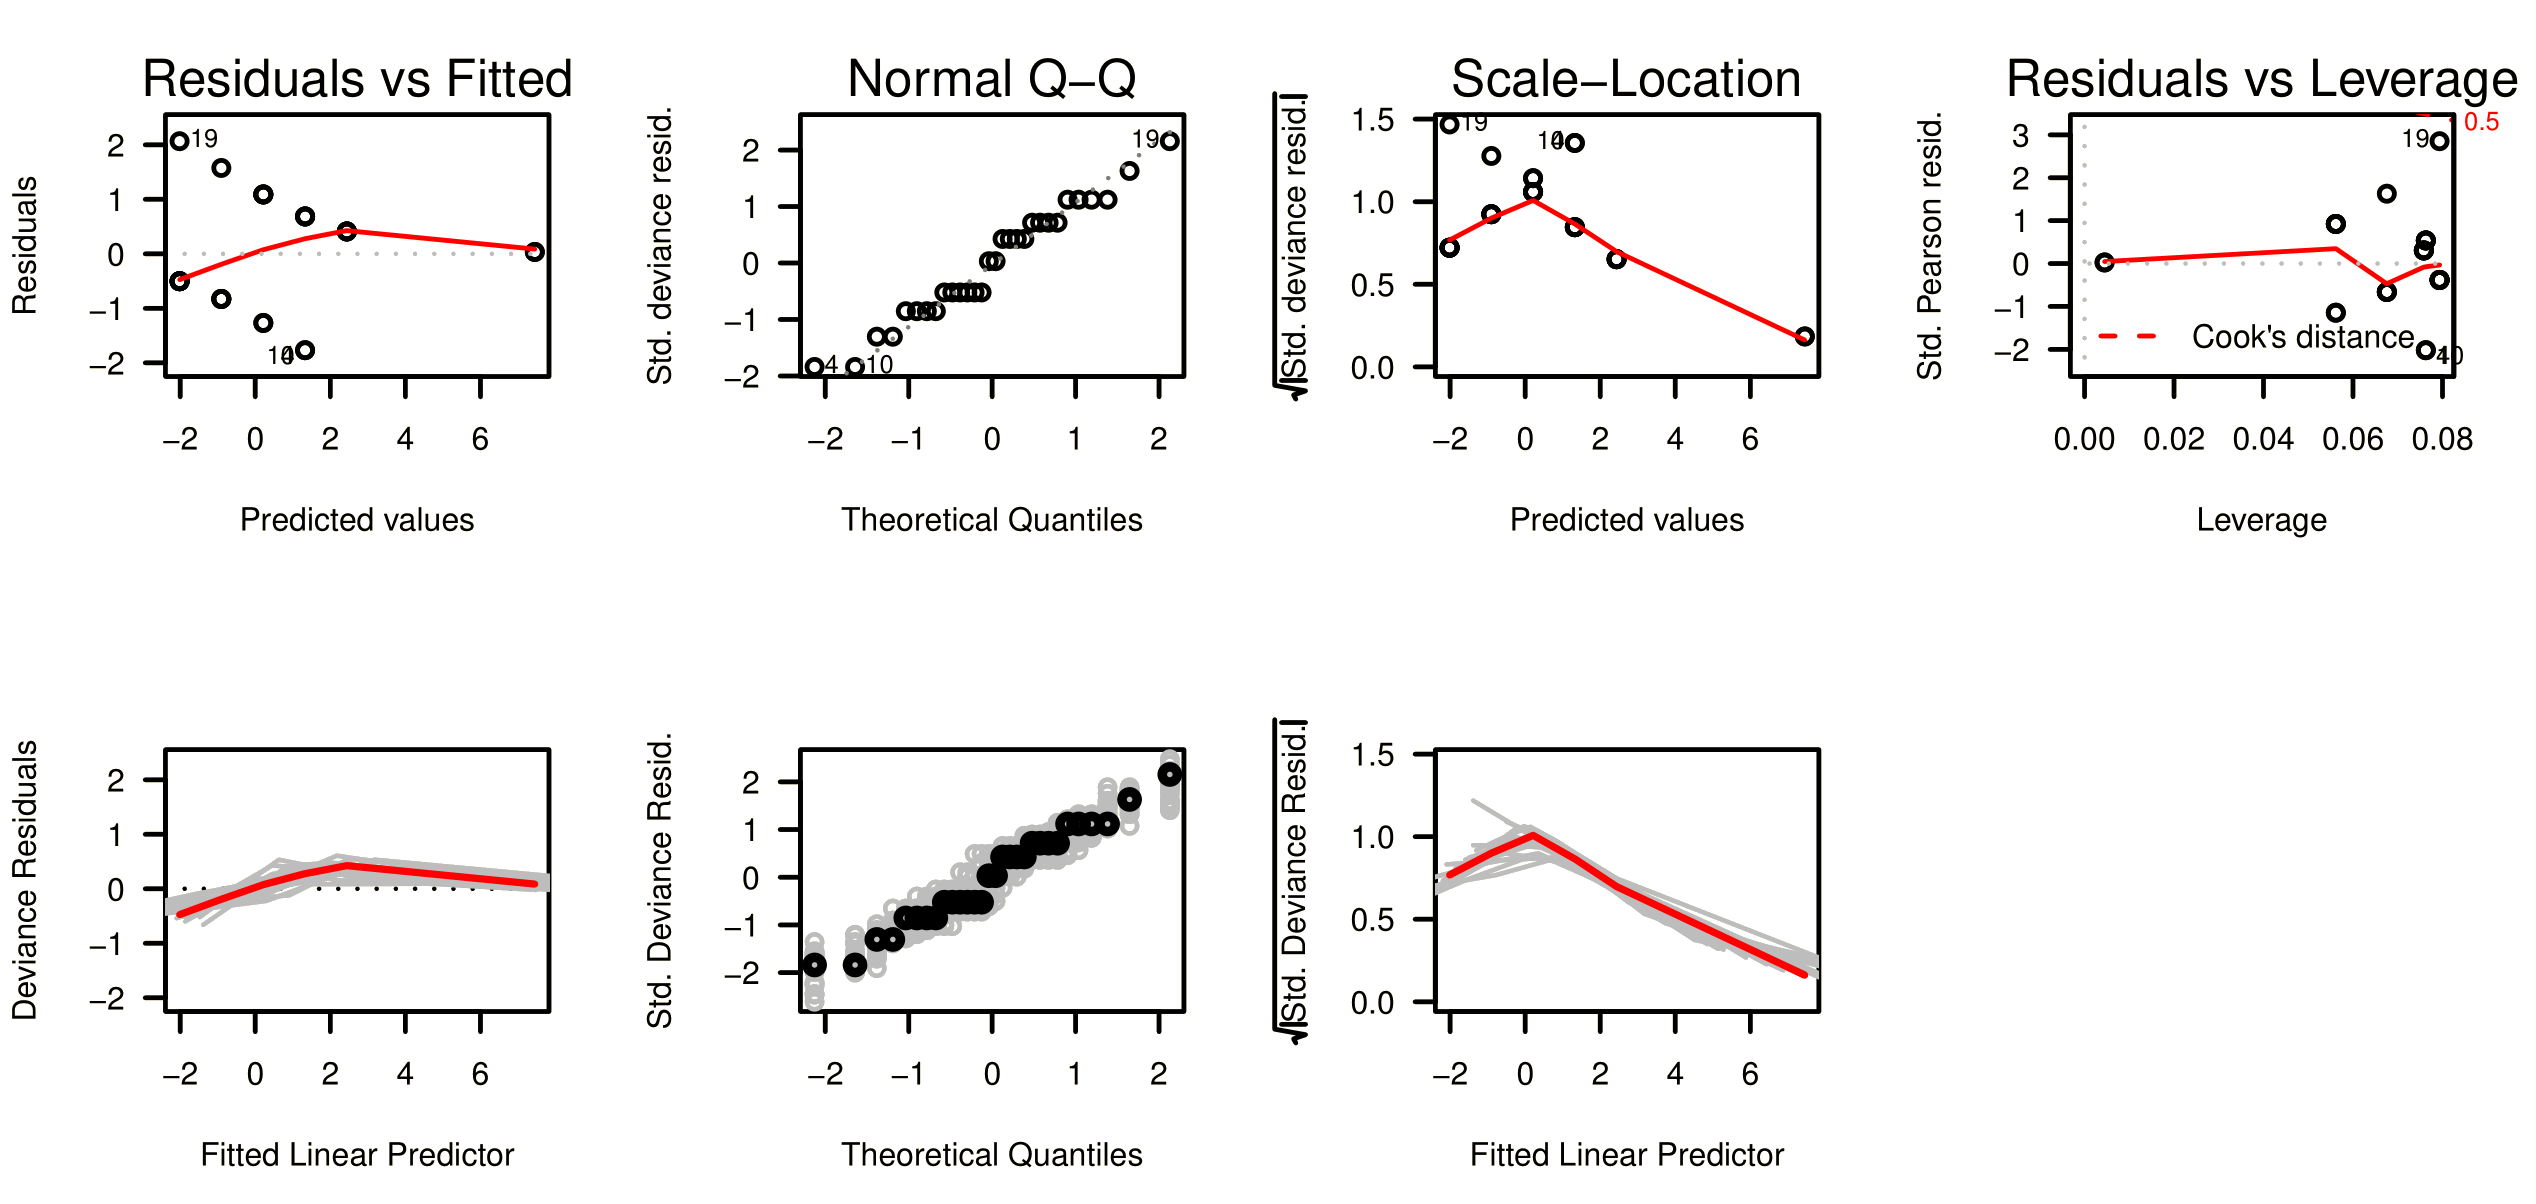
\includegraphics[width=0.9\linewidth, keepaspectratio]{img/glm_diagnostic_plots}
	\caption{Sample plots for a GLM with a binary response (Anesthesia data from the course)}
	\label{fig:glmdiagnosticplots}
\end{figure}

\subsection{Generalised Additive Models}

The generalized additive model (GAM) extends the GLM by replacing some or all of the linear terms of the linear predictor with appropriate smooth functions of the terms

\begin{equation*}
	\eta_i = \beta_0 + \sum_{k=1}^{m} x_i^{(k)}\beta_k\qquad \Rightarrow \qquad \eta_i = \beta_0 + \sum_{k=1}^{m} x_i^{(k)} f_k \left\langle x_i^{(k)} \right\rangle
\end{equation*}

If the response is not Gaussian distributed, the unknown functions can be estimated by the backfitting algorithm where the response $Y_i$ is replaced by the adjusted response and a weighted smoothing is carried out with weights akin to the IRLS algorithm. The \mintinline{R}{mgcv} package takes a likelihood approach, so the implementation of the fitting algorithm is conceptually straightforward.

The main purpose of GAM is to uncover appropriate transformations of explanatory variables. To extract necessary transformations of the explanatory variables from the residual analysis is quite difficult for GLMs. However, GAM are particularly well suited to this, as, according to their structure, they estimate the necessary transformations non-parametrically. The analysis of possibly necessary transformations can thus be done via graphical representations of the estimated functions by superimposing the resulting smooth curve over the partial residual plot.

\begin{figure}[tbh]
	\centering
	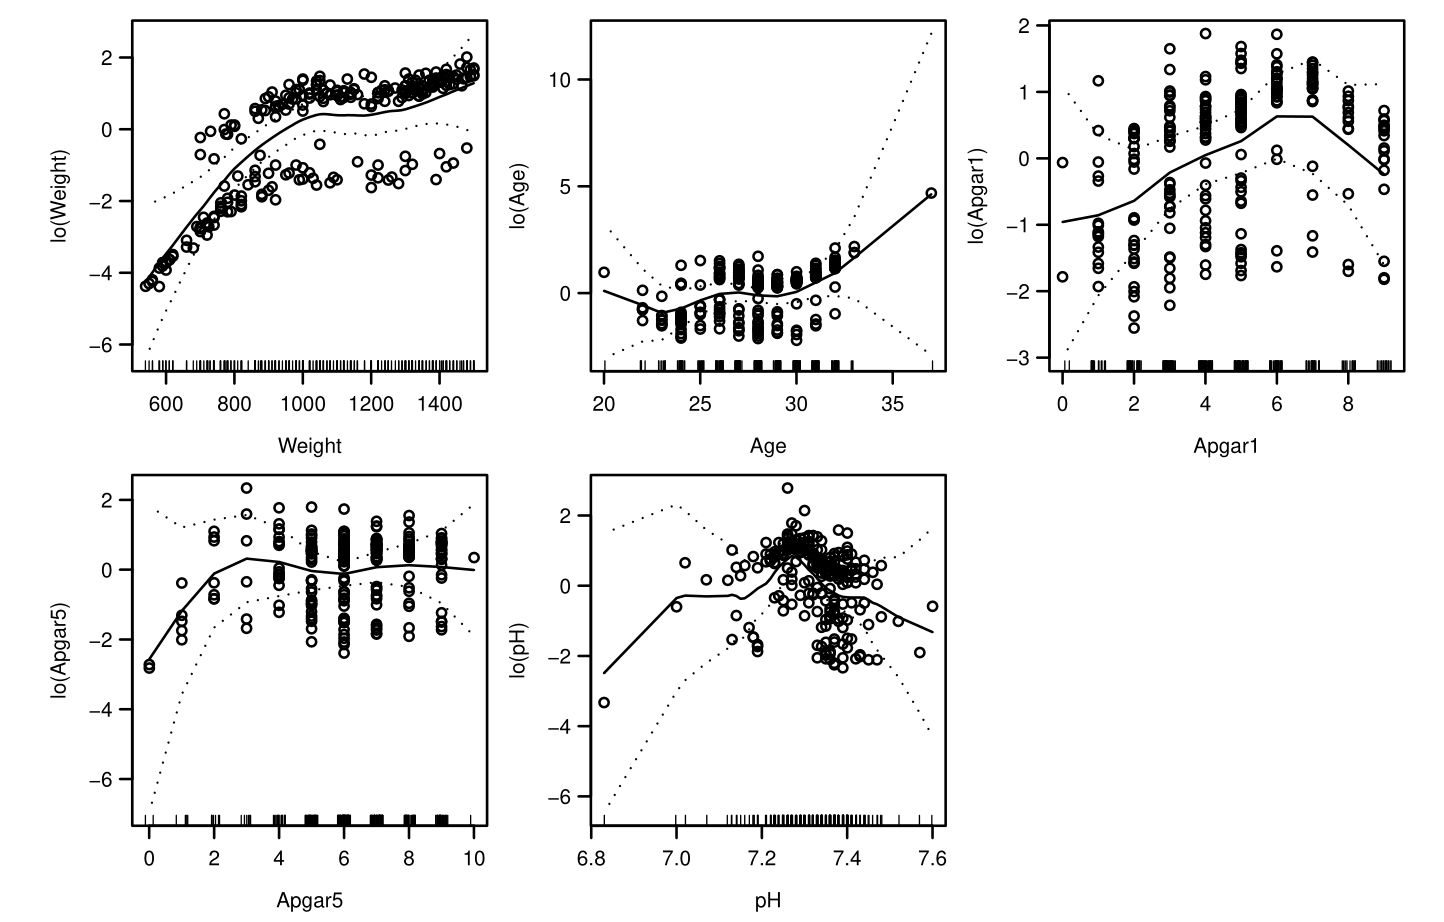
\includegraphics[width=0.8\linewidth, keepaspectratio]{gam_graphical_analysis}
	\caption{Generalised additive model applied to the premature birth data}
	\label{fig:gamgraphicalanalysis}
\end{figure}

\section{Extension of the General Linearised Model}

\subsection{Extension of the Binomial Generalised Linear Model}

Data where the response is a categorical variable with more than two levels can be seen as an extension of the binomial regression model. It's helpful to distinguish between

\noindent
\begin{itemize}[leftmargin=*, labelindent=5cm, labelsep=0.5cm]
	\item[\textbf{nominal multinomial data}] data has no natural order to the response categories
	\item[\textbf{ordinal multinomial data}] data has a natural order to the response categories
\end{itemize}

In both cases there are different types of multinomial models which can be applied to analyse such data which are often collated in a \textbf{contingency table}

\subsection{Contingency Table}

A contingency table is a type of table in a matrix format that displays the (multivariate) frequency distribution of categorical variables.

Contingency table for Party and fAge:
\begin{minted}{R}
> table(USes96$fAge, USes96$Party)
           Democrat   Independent   Republican
(0,25]           33            15           18
(25,35]          76            54           73
(35,45]          89            59           85
(45,55]          68            48           52
(55,65]          49            24           40
(65,75]          41            24           34
(75,100]         24            15           23
\end{minted}

\noindent
The contingency table is best visualised using a \textbf{mosaic plot}

\begin{figure}[H]
	\centering
	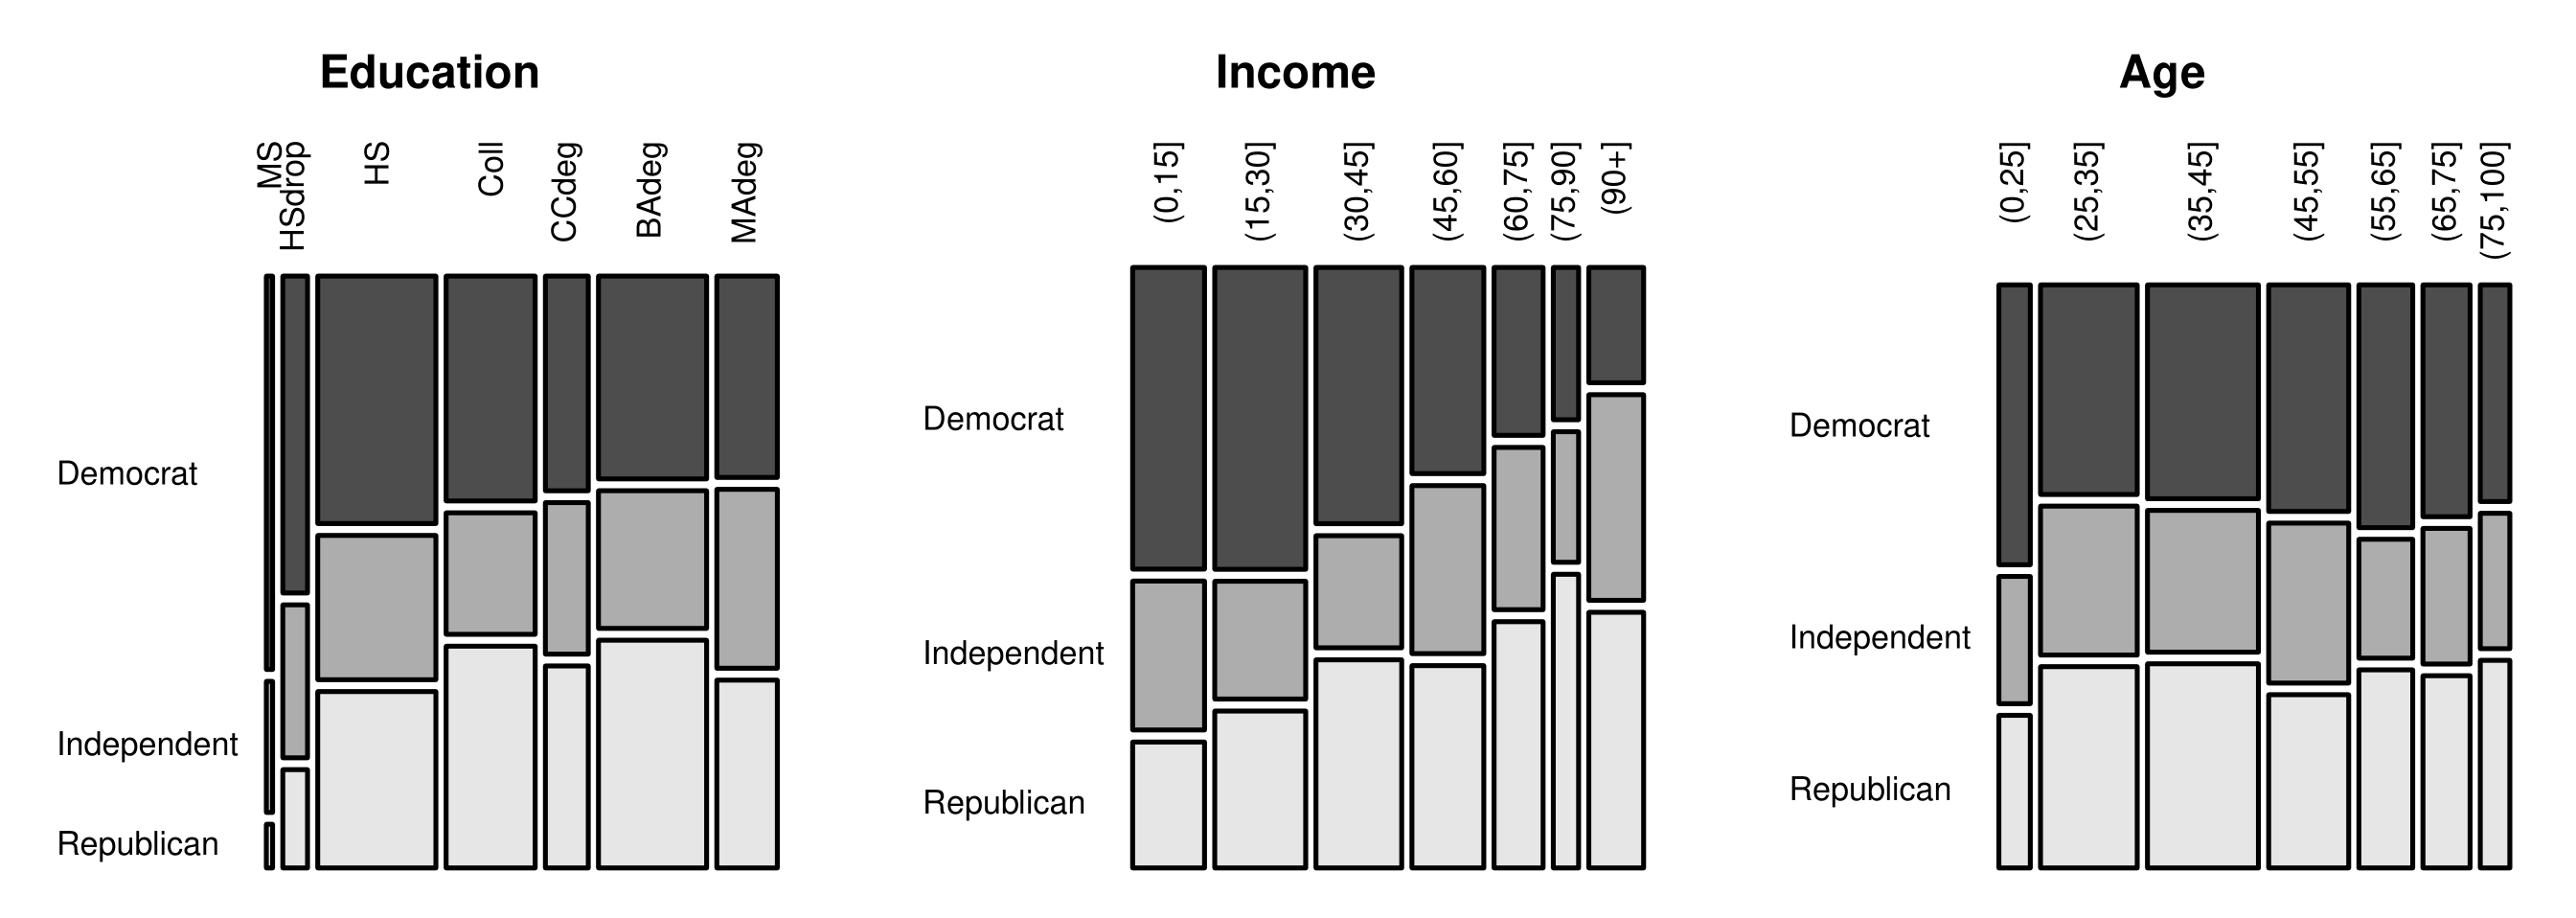
\includegraphics[width=0.9\linewidth, keepaspectratio]{img/mosaic_plot}
	\caption{Mosaic table for the US election study}
	\label{fig:mosaicplot}
\end{figure}

From the marginal distributions in figure \ref{fig:mosaicplot} the conclusion is reached that there are relations between the explanatory variables and the response. The goal is now to include them in a multivariate regression type model to answer whether and which of them are statistically significant.

\subsection{Multinomial Logit Model}

Let $Y_\ell$ be a random variable encoding the response categories with values $1,2,..., L$. Then $\pi_{i\ell} = P\langle Y_i = \ell\rangle$ is the probability that the response of the $i^{\text{th}}$ observation falls into the $\ell^{\text{th}}$ category. And as with binary data, both non-aggregated and aggregated data may be encountered. Thus, let $y_{i\ell}$ be the number of observations falling into category $\ell$, then we can define $ n_i = \sum_{\ell=1}^{L} y_{i\ell}$ as the number of individuals in observation $i$.

The vector $[y_{i1},..., y_{iL}]$ conditioned on the total $n_i$ follows a \textbf{multinomial distribution}

\begin{equation*}
	P\left\langle Y_{i1}=y_{i1}, Y_{i2}=y_{i2}, ... , Y_{iL}=y_{iL} | \sum_{\ell=1}^{L} y_{i\ell} = n_i \right\rangle = \frac{n_i !}{y_{i1}!y_{i2}!\cdots y_{iL}!} \pi_{i1}^{y_{i1}}\pi_{i2}^{y_{i2}}\cdots\pi_{iL}^{y_{iL}}
\end{equation*}

The goal will again be to find a relation between the probabilities $[ \pi_{i1},...,\pi_{iL} ]$ and the explanatory variables $x_i$. The idea applied is similar to the one used in the logit model:

\begin{equation*}
	\log\left\langle \frac{P\left\langle Y_{i\ell}=y_{i\ell}\middle| \underline{x}_i\right\rangle}{P\left\langle Y_{i1}=y_{i1}\middle| \underline{x}_i\right\rangle} \right\rangle = \log\left\langle\frac{\pi_{i\ell}}{\pi_{1\ell}}\right\rangle = \eta_{i\ell} = \beta_{0\ell} + \beta_{1\ell}x_i^{(1)} + \cdots + \beta_{m\ell}x_i^{(m)}\qquad\forall\ell=2,3,...,L
\end{equation*}

\subsubsection{Example Multinomial Analysis}

\begin{minted}[breaklines, fontsize=\small]{R}
> library(nnet)
> USes96.mn <- multinom(Party ~ fAge + income + educ, data=USes96)
# weights: 60 (38 variable)
initial value 1037.090001
iter 10 value 982.279778
iter 30 value 976.100827
final value 976.098800
converged

> summary(USes96.mn)
Call:
multinom(formula = Party ~ fAge + income + educ, data = USes96)

Coefficients:
               (Intercept)   fAge(25,35]    fAge(35,45]    fAge(45,55]    fAge(55,65]
Independent     -0.4614714     0.2427764     0.08627062    -0.02159704     -0.1652051
Republican      -0.5740834     0.3658397     0.22536875    -0.10183031      0.2641415
.
. ....

Std. Errors:
               (Intercept)   fAge(25,35]    fAge(35,45]    fAge(45,55]    fAge(55,65]
Independent      0.3492804     0.3691652      0.3674895      0.3844265      0.4166222
Republican       0.3543365     0.3501576      0.3471449      0.3694353      0.3834749
.
. ....

Residual Deviance: 1952.198
AIC: 2028.198
\end{minted}

For inferring whether the $k^{\text{th}}$ explanatory variable has a significant impact on the response, individual hypothesis tests are not possible any more and one has to resort to a comparison of nested models based on deviance differences.

\begin{minted}[breaklines, fontsize=\small]{R}
> USes96.mn2 <- multinom(Party ~ fAge + income, data=USes96)
# weights: 42 (26 variable)
initial value 1037.090001
iter 10 value 986.500046
iter 30 value 983.790955
final value 983.790553
converged
> (h1 <- deviance(USes96.mn2)-deviance(USes96.mn)) # difference of deviances
[1] 15.38351
> (h2 <- abs(USes96.mn2$edf - USes96.mn$edf)) # difference of df
[1] 12
> pchisq(h1, h2, lower=FALSE) # p-value calculation
[1] 0.2211305
\end{minted}

And to obtain predicted probabilities

\begin{minted}[breaklines, fontsize=\small]{R}
> round(predict(USes96.mn2, type="probs"),3)[1:10,]
> h3 <- c(353, 369, 34, 300, 503, 467, 332, 817, 437, 385)
       Democrat    Independent    Republican
353       0.482          0.163         0.356
369       0.382          0.202         0.416
34        0.503          0.276         0.221
300       0.474          0.216         0.310
503       0.482          0.163         0.356
467       0.411          0.209         0.380
332       0.474          0.216         0.310
817       0.262          0.224         0.514
437       0.482          0.163         0.356
385       0.516          0.200         0.284
\end{minted}

\paragraph{Note} Up until today, there is no meaningful definition of what residuals are in the context of the multinomial logit model. There are some for each of the $(L-1)$ equations in the system, and they also depend on the choice of the baseline category. How these could be displayed in a comprehensive form is unclear. Thus there is no effective tool for model enhancement.

\subsection{Ordinal Multinomial Response}

For ordinal multinomial models, the response is still categorical with $L\geq 2$, but there is a natural ordering among the categories too (refer to figure \ref{fig:mentalimpairment}).

\begin{figure}[tbh]
	\centering
	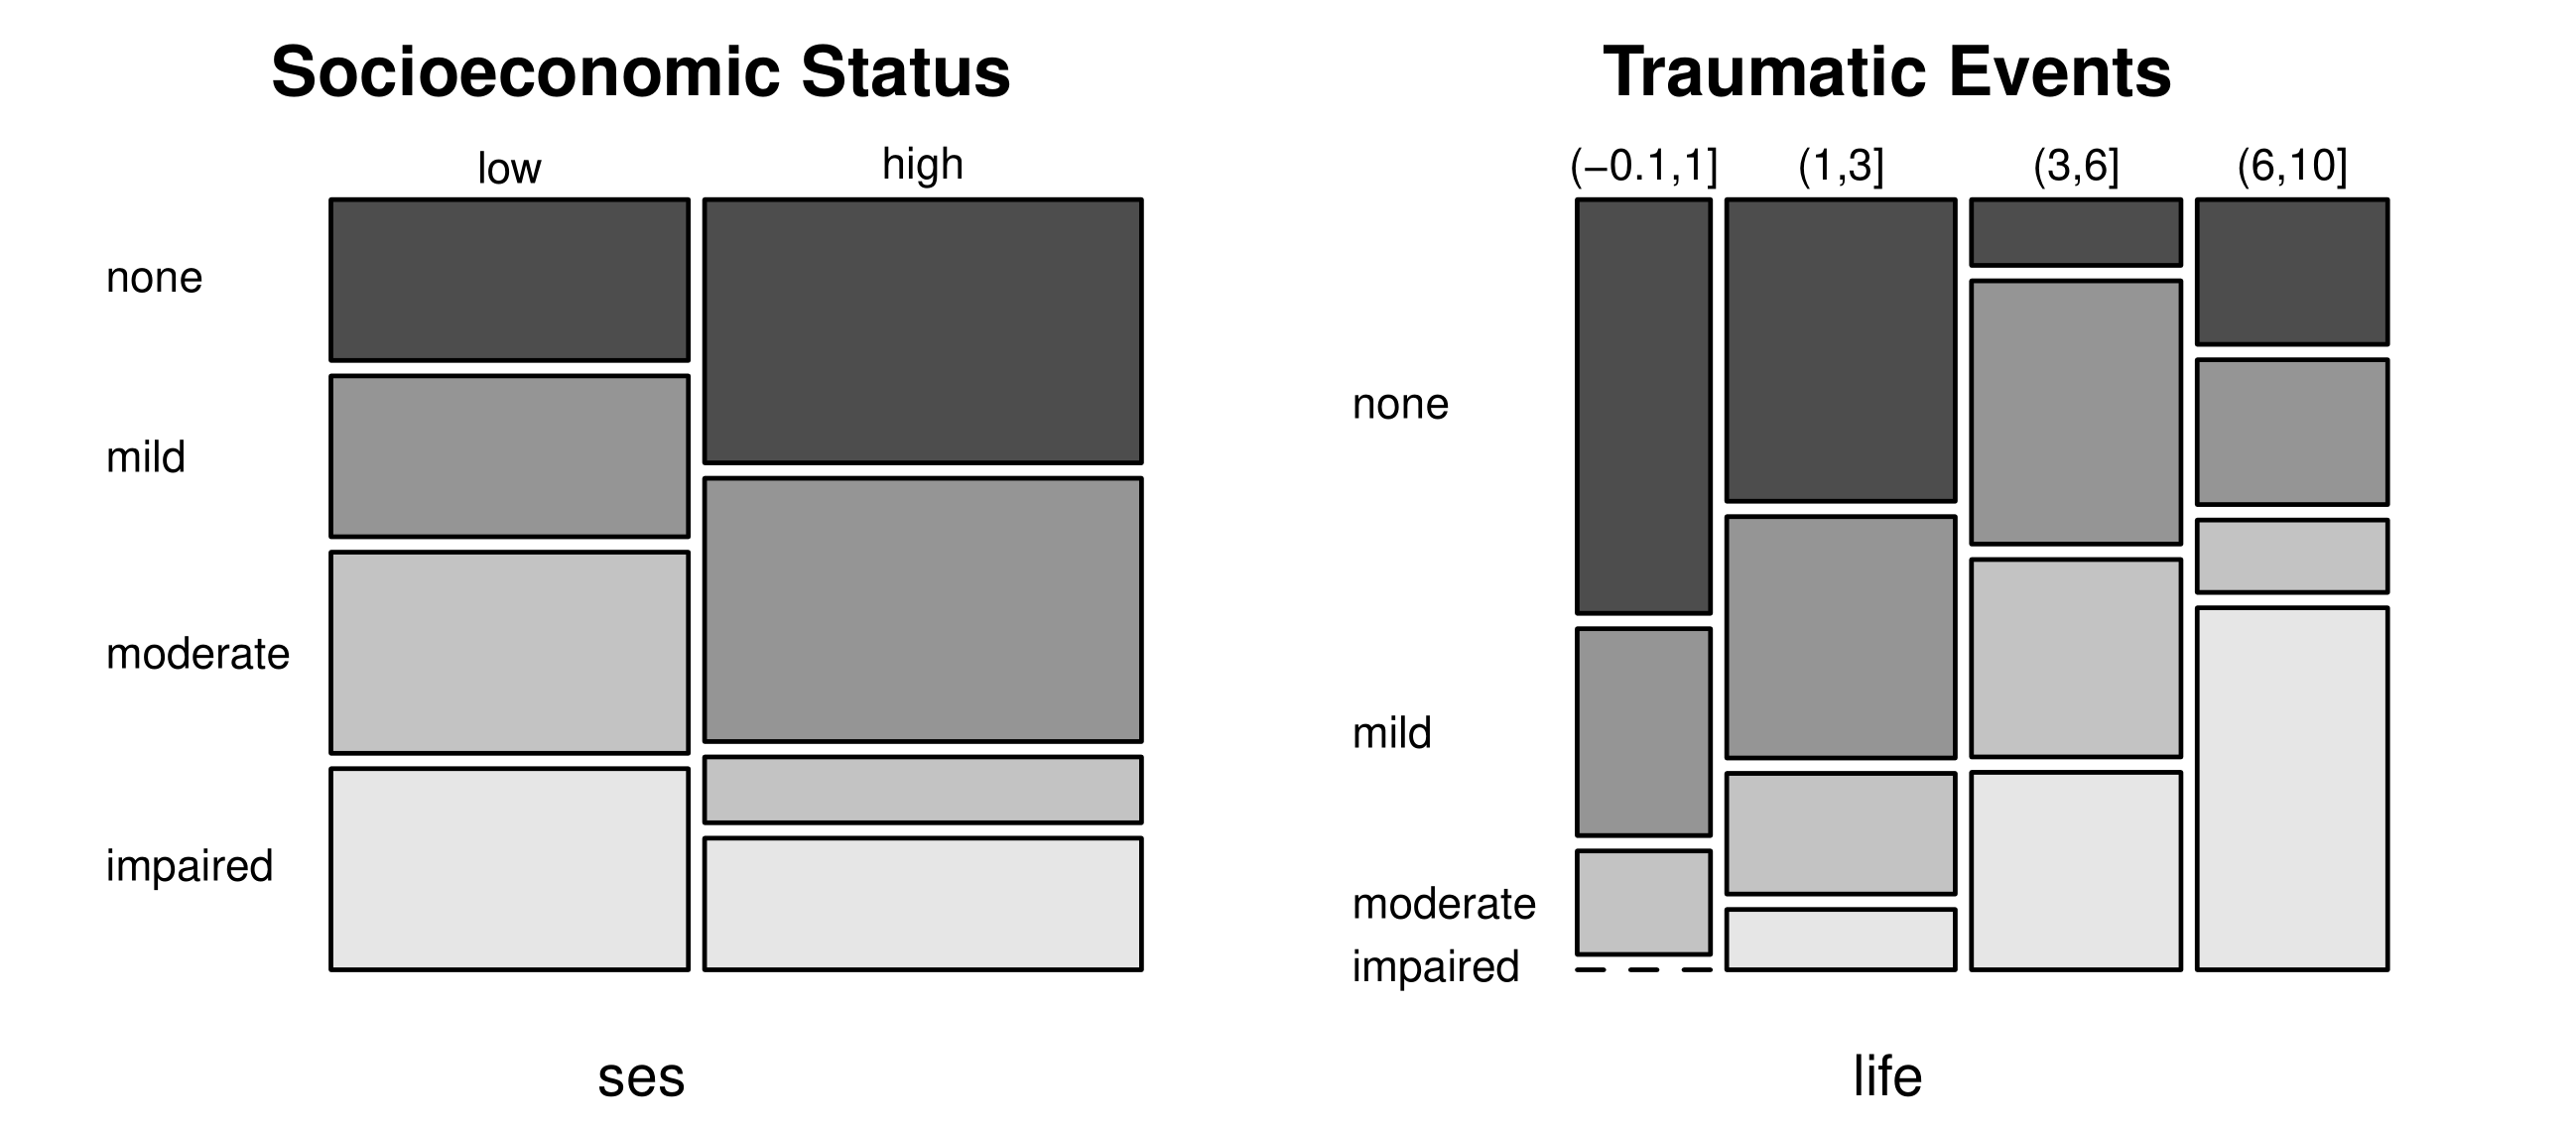
\includegraphics[width=0.8\linewidth, keepaspectratio]{img/mental_impairment}
	\caption{Mental impairment in relation to status and number of events}
	\label{fig:mentalimpairment}
\end{figure}

With an ordered response, it is often easier and more powerful to work with cumulative probabilities

\begin{equation*}
	\gamma_{i\ell} = P\langle Y_i\leq\ell\rangle
\end{equation*}
with $\gamma_{iL} = 1$, so we need only model $(L-1)$ probabilities.
Considering three possibilities which all take the form $g\langle\gamma_{i\ell}\rangle = \alpha_\ell - \underline{x}_i^T\underline{\beta}$, where $g\langle \cdot \rangle$ can be the usual logit, probit or the complementary log-log. Note that the regression coefficients $\beta$ do not depend on the class $\ell$ and thus, the explanatory variables have some uniform effect on the response categories.

\begin{minted}[breaklines, fontsize=\small]{R}
> Mental$sLE <- sqrt(Mental$life)
> library(MASS)
> mi.polr <- polr(impair ~ ses + sLE, data=Mental)
> summary(mi.polr)

Re-fitting to get Hessian

Call:
polr(formula = impair ~ ses + sLE, data = Mental)
Coefficients:
             Value    Std. Error    t value
seshigh     -1.104        0.6095     -1.811
sLE          1.143        0.4577      2.498
Intercepts:
                      Value    Std. Error    t value
none|mild            0.5950        0.9347    0.6366
mild|moderate        2.0790        0.9816    2.1179
moderate|impaired    3.0617        1.0395    2.9452

Residual Deviance: 99.45508
AIC: 109.4551
\end{minted}

Instead of performing multiple single hypothesis tests, it is preferable to run deviance tests for nested models.

\begin{minted}[breaklines, fontsize=\small]{R}
> anova(mi.polr, mi.polr2)
Likelihood ratio tests of ordinal regression models
Response: impair
        Model   Resid. df    Resid. Dev      Test    Df     LR stat.      Pr(Chi)
1         sLE          36     102.85013
2   ses + sLE          35      99.45508    1 vs 2     1     3.395051   0.06539236
\end{minted}

With a p-value of 0.065 there is no statistical evidence on a 5\% level that the socioeconomic status should be included in the model. To predict values with the constructed model

\begin{minted}[breaklines, fontsize=\small]{R}
> predict(mi.polr2, type="probs")[1:6,]
          none         mild     moderate      impaired
1    0.5031476    0.2992945   0.10799478    0.08956314
2    0.1141223    0.2265565   0.22324007    0.43608113
3    0.7395325    0.1797455   0.04682456    0.03389745
4    0.2653472    0.3262757   0.19219086    0.21618620
5    0.3225415    0.3337747   0.17064951    0.17303429
6    0.3978473    0.3281870   0.14294305    0.13102257

> predict(mi.polr2, type="class")[1:6]
[1] none impaired none mild mild none
Levels: none mild moderate impaired
\end{minted}

As is the case for the multinomial logit model of unordered responses, there is no useful definition of residuals that would allow for model enhancement through diagnostics for this model class.

\section{Bayesian Data Analysis}

In the frequentist domain we assume that the underlying probability stays the same, this is not true in the real world. In Bayesian data analysis the goal is to understand the underlying \textbf{data generating process} or \textbf{generative model}. 

In the classical statistical approach the assumption is, that for a given generative model the parameters are unknown but fixed and observed data is random.

\paragraph{Example - Election model} You want to predict the result of an election, you ask 120 randomly chosen people about their preference: 68 prefer party A, 52 prefer party B. The estimation with maximum likelihood ($\max P(D|\theta)$)
\begin{equation*}
	p = \frac{68}{120}
\end{equation*}

Approximate 95\% confidence interval:
\begin{minted}{R}
> sim = rbinom(10000, 120, p)/120
> quantile(sim, c(0.025, 0.975))
> qbinom(c(0.025,0.975),120,p)/120
> binom.test(68, 120, p=0.5) # two-sided!
# p-Value
> length(sim[sim<=0.5])/10000
> binom.test(68, 120, p=0.5, alternative="greater")
\end{minted}

In a Bayesian approach, for a given (generative) model there is uncertainty and respectively variation of belief about the parameters of the model. Observed data is fixed and not random at all. In the Bayesian approach the uncertainty about the model parameters get modelled with probability. The prior belief about the generative model get stated explicitly. A prior consistent with the Frequentist approach is a uniform distribution. Fortunately the prior belief gets more and more irrelevant with increasing data. Neglecting prior information or modelling uninformative prior information results in the special case of the classical statistical approach, with exploiting the likelihood function.

\begin{figure}[tbh]
	\centering
	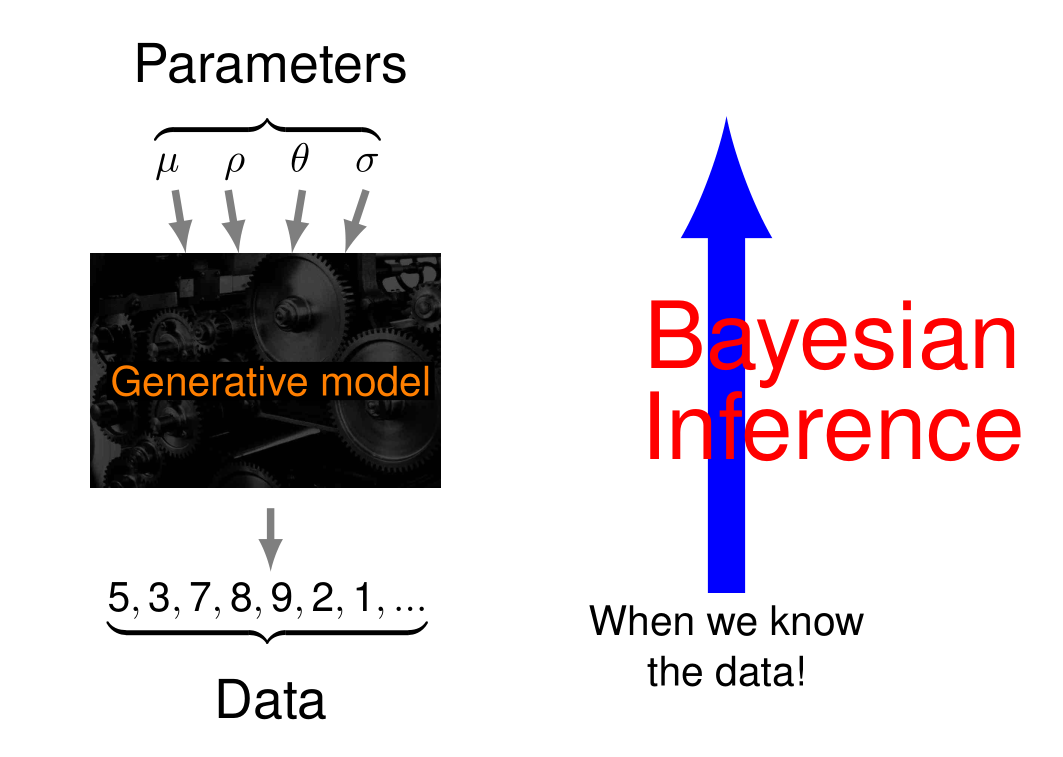
\includegraphics[width=0.6\linewidth, keepaspectratio]{img/bayesian_approach}
	\caption{The Bayesian approach}
	\label{fig:bayesianapproach}
\end{figure}

\noindent
To perform a Bayesian data analysis one needs
\begin{itemize}
	\item observed \textbf{data} to draw conclusions from
	\item a \textbf{generative model} or data generating process
	\item to quantify the underlying uncertainty of the parameters in the model, that is to include \textbf{prior information} before looking at the data
\end{itemize}

With a clear understanding of the random process leading to the data, a Bayesian data analysis is done in three steps:
\begin{enumerate}
	\item Set up a full probability model and include all types of uncertainty
	\item Apply a condition on the observed data and filter accordingly
	\item Evaluate the fit of the model and implications on posterior distribution
\end{enumerate}

\paragraph{Example - Swedish Fish Inc.} The company wants to enter the Swiss market, they send a catalogue with a sample to 16 people, with 6 of them signing up. 
\begin{itemize}
	\item \textbf{Observed data}: 6 out of 16 signed up
	\item \textbf{Generative model}: There is a certain fraction $\theta$ of people in the population, that would be willing to sign up. Thus, the probability that a randomly chosen person signs up is $\theta$. This is like tossing a coin with success probability $\theta$.
\end{itemize}

There is a certain subjective component in a Bayesian analysis, that reflects your \textbf{state of belief} and \textbf{initial assumptions}.

Often, this \textbf{subjective belief} is the origin of doubt on Bayesian methods. However, you can use uninformative priors or try out different priors and \textbf{examine the influence of your assumptions} on the results of your analysis.

Fortunately, the more data you have, the less important your prior information gets.

Assume, we have \textbf{no information} about the sign-up rate. We don’t want to include any bias or assumptions on $\theta$, that could influence our analysis. For this we assume that $\theta$ is uniformly distributed between 0 and 1:
\begin{equation*}
	\theta\sim\text{Uniform}(0,1)
\end{equation*}

A uniform prior is often called uninformative prior, because it includes no preferences and doesn't favour one value over another.

\begin{figure}[htb]
	\begin{subfigure}{.5\textwidth}
		\centering
		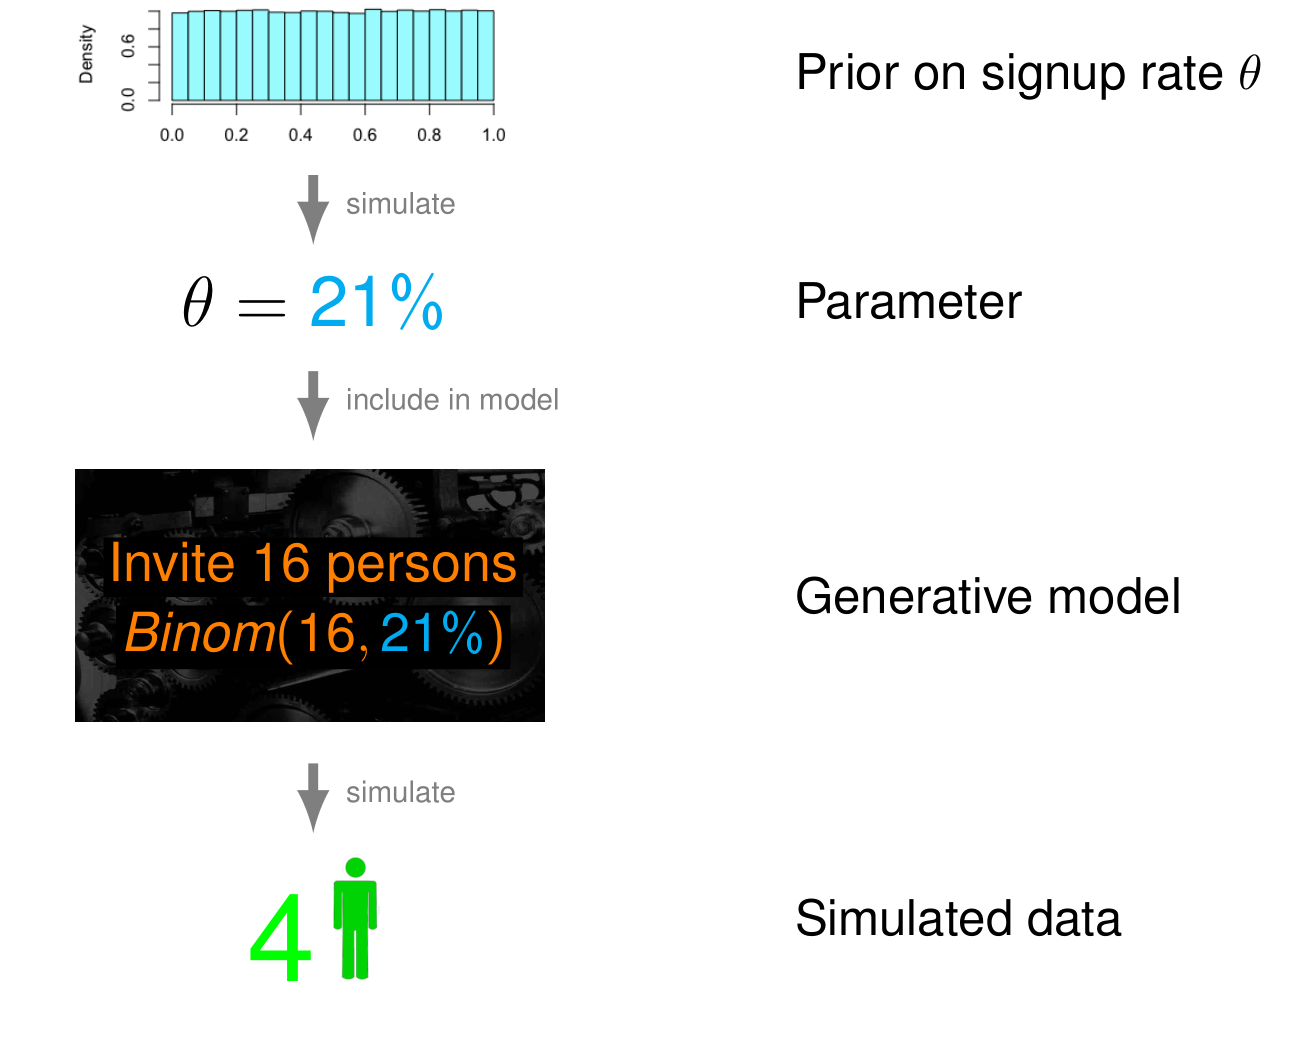
\includegraphics[width=0.7\linewidth, keepaspectratio]{img/bayesian_approach_simulation}
		\caption{Simulation of data using the generative model}
		\label{fig:bayesianapproachsimulation}
	\end{subfigure}
	\begin{subfigure}{.5\textwidth}
		\centering
		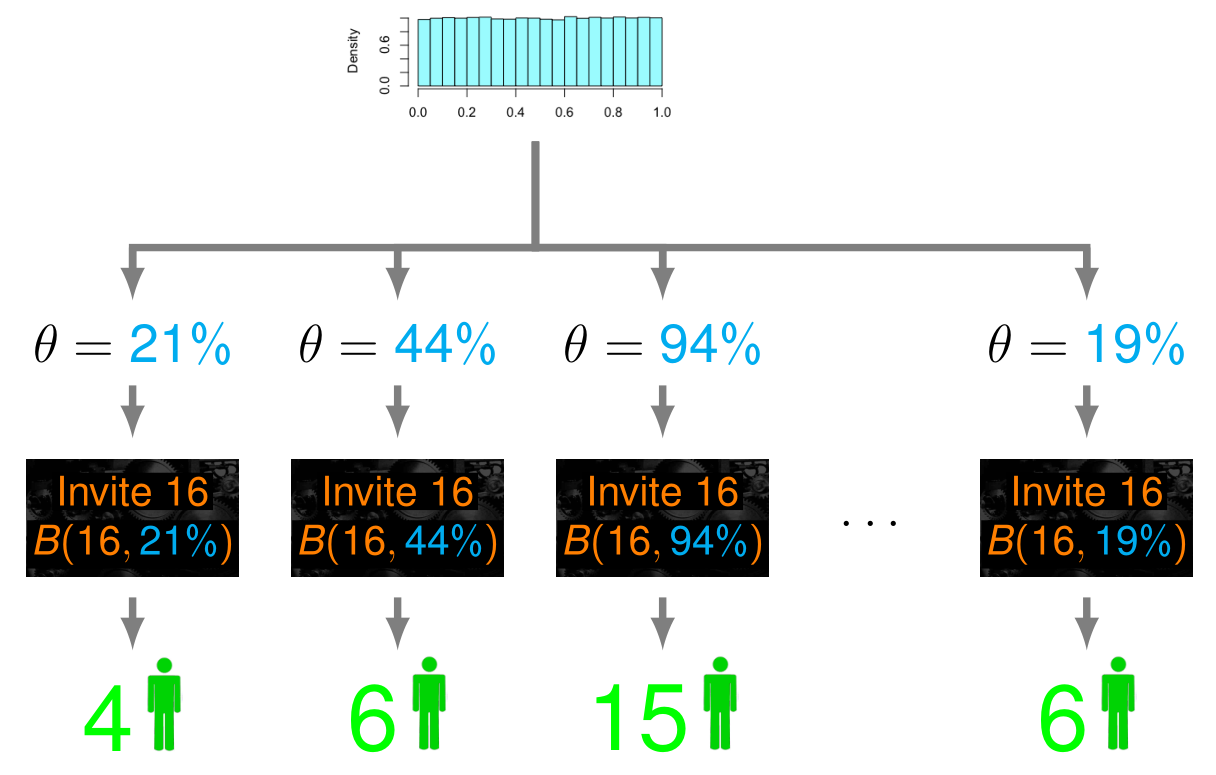
\includegraphics[width=0.9\linewidth, keepaspectratio]{img/bayesian_approach_repeated_simulation}
		\caption{Repeated simulations}
		\label{fig:bayesianapproachrepeatedsimulation}
	\end{subfigure}
\end{figure}

\begin{minted}[linenos]{R}
n = 10000
nInvited = 16
nSignups = 6
prior = runif(n,0,1) # Here you sample n draws from the prior
hist(prior) # It’s always good to eyeball the prior to make sure it looks ok
# Define the generative model:
	generativemodel = function(theta){
	rbinom(1,nInvited,theta)
}
# Simulate data using parameters from the prior and the generative model:
simdata = rep(NA, n)
for(i in 1:n) {
	simdata[i] = generativemodel( prior[i] )
}
# Filter out all draws that do not match the data:
posterior = prior[simdata == nSignups]
hist(posterior) # Eyeball the posterior
length(posterior) # Are there enough draws left after the filtering?
# There are no rules here, but you probably want to aim for >1000 draws.
\end{minted}

\begin{figure}[hb]
	\centering
	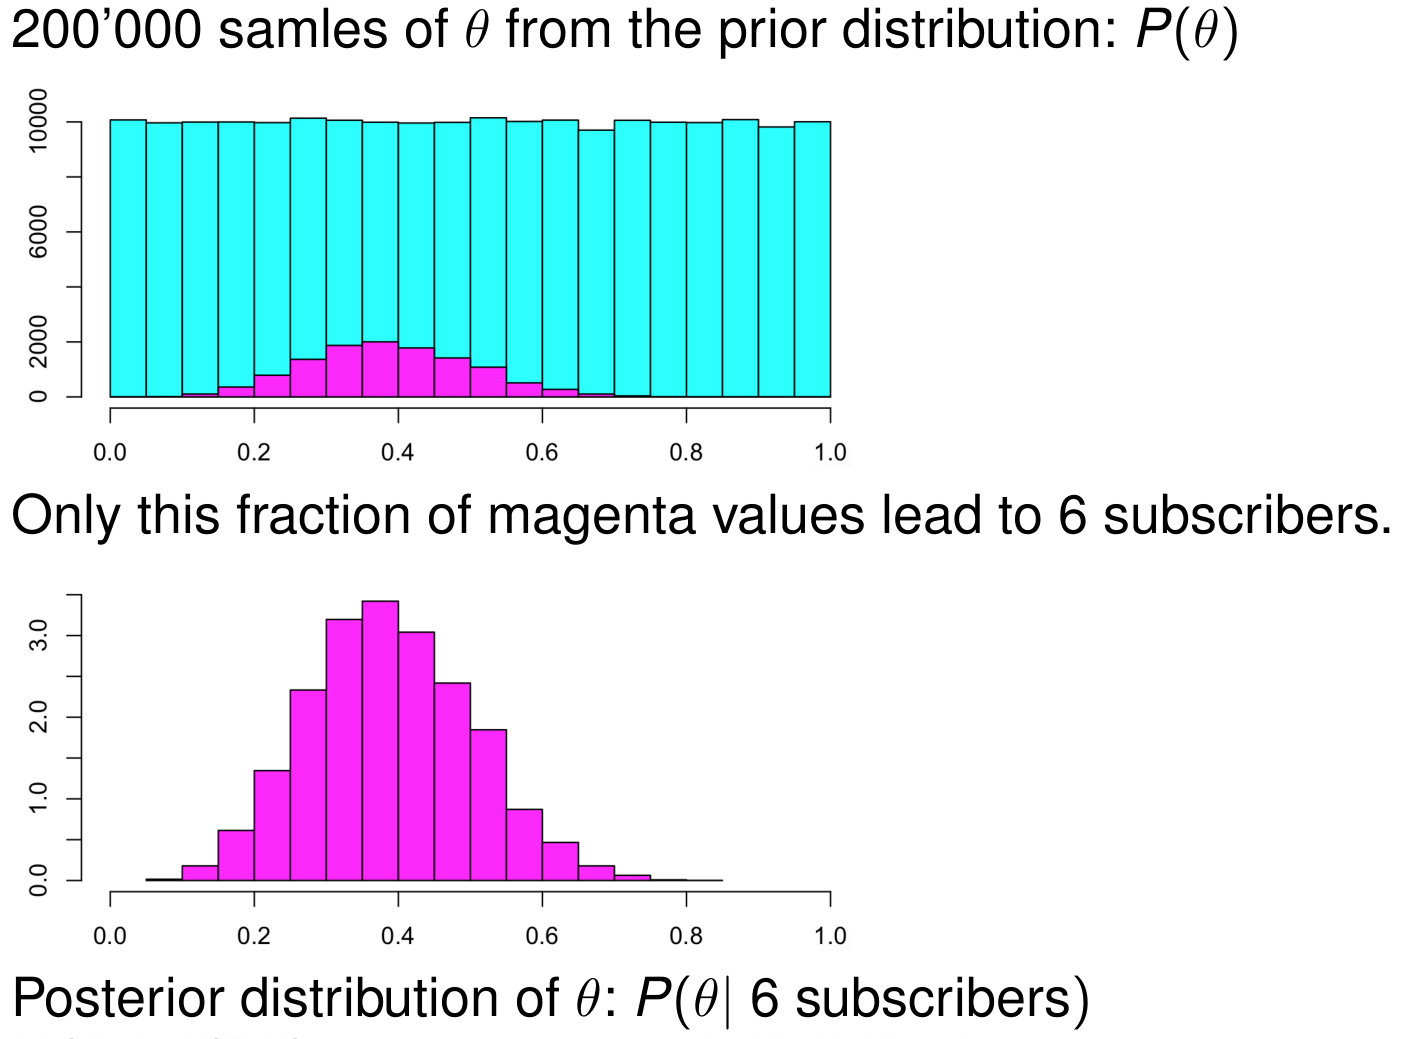
\includegraphics[width=0.6\linewidth, keepaspectratio]{img/effect_sampling_posterior}
	\caption{Effect of the simulation on the posterior distribution}
	\label{fig:effectsamplingposterior}
\end{figure}

As seen in figure \ref{fig:evaluationposteriordistribution}, the mean calculated by the Bayesian analysis is $0.389961$ compared to the MLE of $0.375$.

\begin{minted}{R}
> quantile(posterior,c(0.05,0.95))
[1] 5% 95%
[2] 0.2139047 0.5822077
> mean(posterior)
[1] 0.389961
\end{minted}

\begin{figure}[tbh]
	\centering
	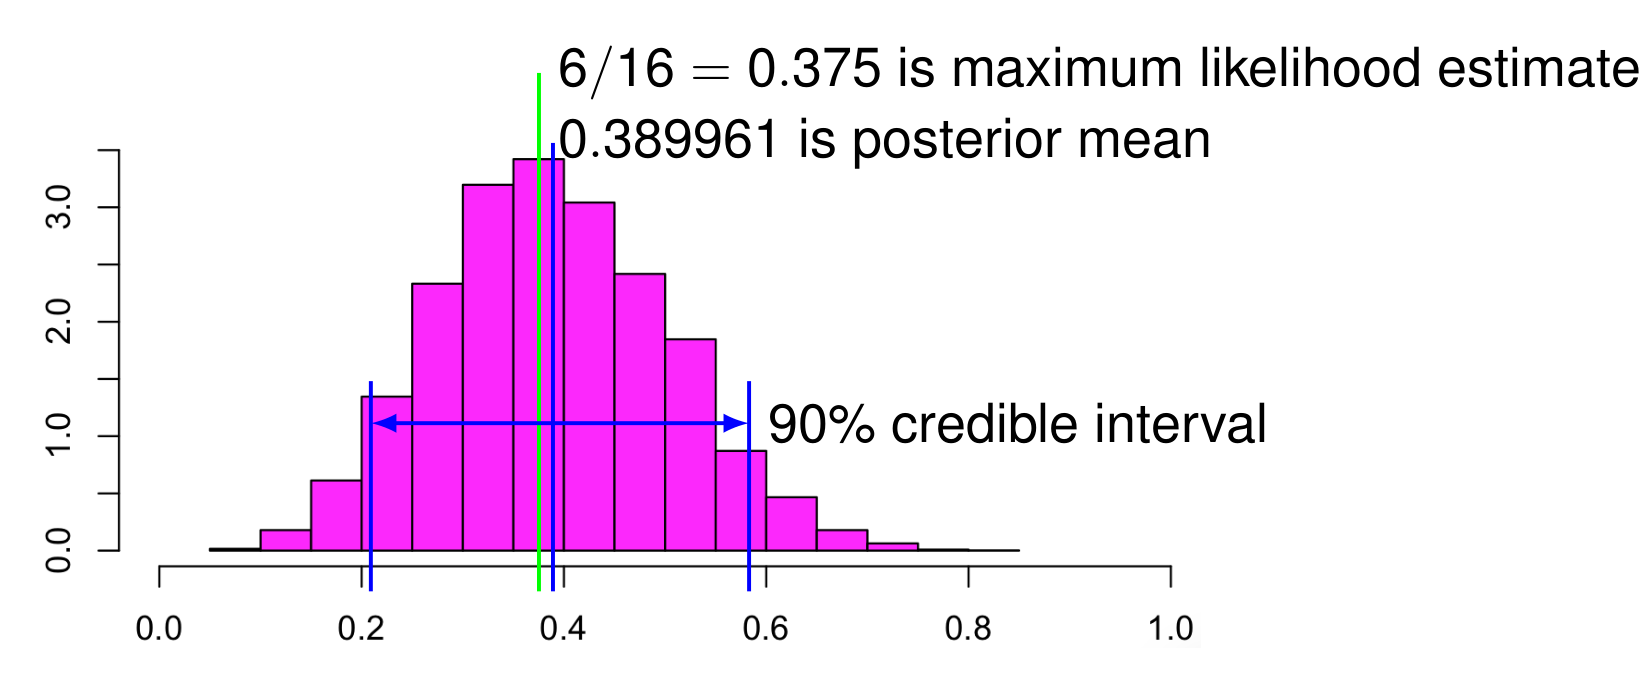
\includegraphics[width=0.6\linewidth]{img/evaluation_posterior_distribution}
	\caption{Evaluation of the posterior distribution}
	\label{fig:evaluationposteriordistribution}
\end{figure}

\subsection{Credible Intervals}

Credible intervals are not unique. Suitable intervals are:

\begin{enumerate}
	\item The \textbf{highest posterior density interval (HDI)} contains the values with highest probability density. For a unimodal distribution it’s the narrowest possible credible interval. It contains all values up to a certain probability threshold.
	\item For the \textbf{equal-tailed interval} the probability of being below the interval is as likely as being above it. You get this by just trimming both ends.
\end{enumerate}

Remark: A frequentist 95\% confidence interval means that with a large number of repeated samples, 95\% of such calculated confidence intervals would include the true value of the parameter. In frequentist terms, the parameter is fixed and the confidence interval is random.

\subsection{Modelling Prior Belief About $\theta$}

The exact value of $\theta$ is not known and there is thus uncertainty about this parameter. To model prior knowledge about $\theta$ before seeing the observed data, it is possible to explicitly state this belief and introduce it into the model.

Assume, there is some information or expert knowledge about the sign-up rate which should be included in the model.

The beta distribution has its support on $[0,1]$ and has two parameters to adjust the mean and shape of the distribution. So the beta distribution is a good choice to model the prior belief on $\theta$.

\subsubsection{Beta Distribution}
\begin{minipage}{\textwidth}
	\renewcommand{\arraystretch}{1.5}
	\centering
	\begin{tabularx}{\textwidth}{r X X}
		\hline
		& \textbf{Description} & \textbf{Notes}\\
		\hline
		$ X \sim \text{Beta}(a,b)$ & Notation & $a$ and $b$ are shape parameters\\
		$[0,1]$ & Support of the Beta distribution & \\
		$ p(x|a,b) = \left\{ \begin{matrix}
		\frac{\Gamma(a+b)}{\Gamma(a)\Gamma(b)} x^{a-1}(1-x)^{b-1} &0<x<1\\
		0 & \text{else}
		\end{matrix} \right. $ & Probability density function & $\Gamma(n) = (n-1)!$\\
		$\mathbb{E}(X) = \frac{a}{a+b}$ & Mean & \\
		$\text{Var}(X) = \frac{a\cdot b}{(a+b+1)(a+b)^2}$ & Variance & \\
		$\text{mode}(X) = \frac{a-1}{a+b-2} \quad\text{for }a,b>1$ & Mode & The mode of a set of data values is the value that appears most often\\
	\end{tabularx}
\end{minipage}

See figure \ref{fig:betadistributionparameters} for plots of different beta distributions.

\begin{figure}[tbh]
	\centering
	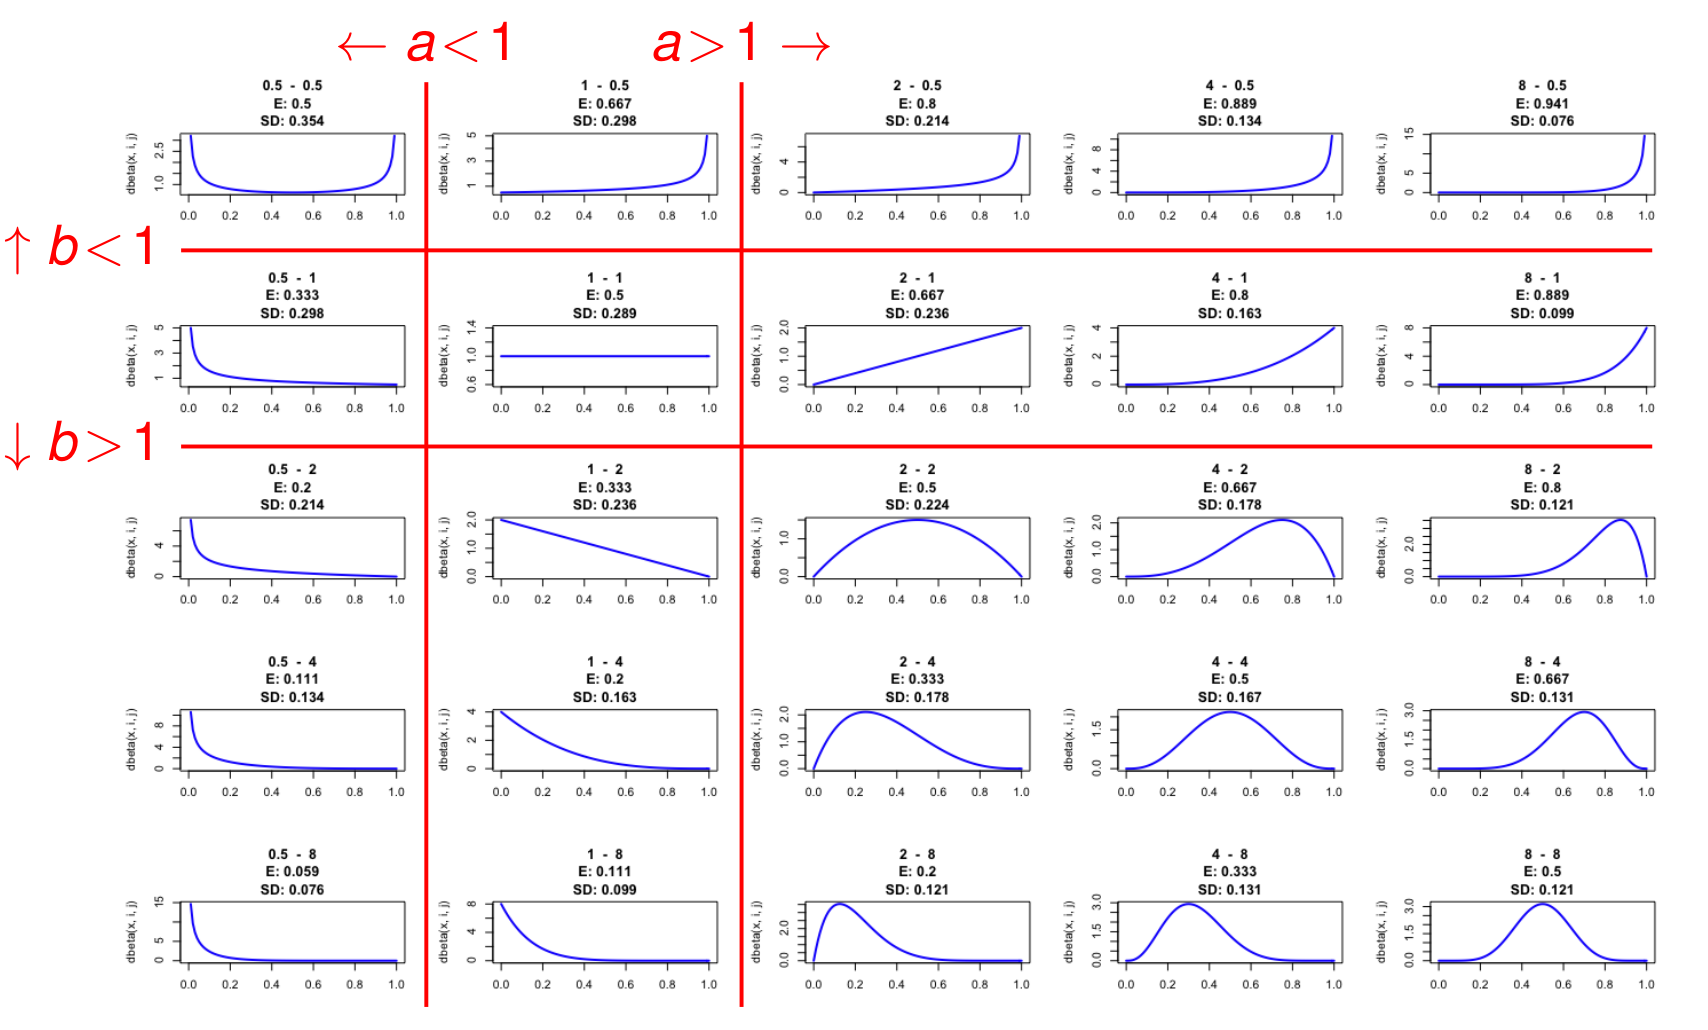
\includegraphics[width=\linewidth, keepaspectratio]{img/beta_distribution_parameters}
	\caption{Beta distribution with different values for $a,b$}
	\label{fig:betadistributionparameters}
\end{figure}

\subsection{Summary On Inferring The Sign-Up Rate $\theta$}

A Bayesian data analysis transforms the prior into the posterior distribution of parameters, by including observed data.

Different priors lead to different posterior distributions. In the preceding example there was only few data, so the impact of the prior on the posterior was high. And the more data there is, the less important the prior gets.

With a uniform prior, the posterior distribution is proportional to the likelihood function $P(\theta|D)$, which is used in classical statistics. In this sense Bayesian analysis is a generalisation of the Frequentists approach. In a Bayesian setting there are not just point estimates, instead the uncertainty is preserved and can be used for further considerations.

\section{Approximate Bayesian Computation (ABS)}
The \textbf{conditional probability} $P(A|B)$ is the probability of A given B has occurred.
\begin{equation*}
	P(A|B) = \frac{P(A\cap B)}{P(B)}
\end{equation*}

\noindent
\begin{minipage}{0.3\linewidth}
	\centering
	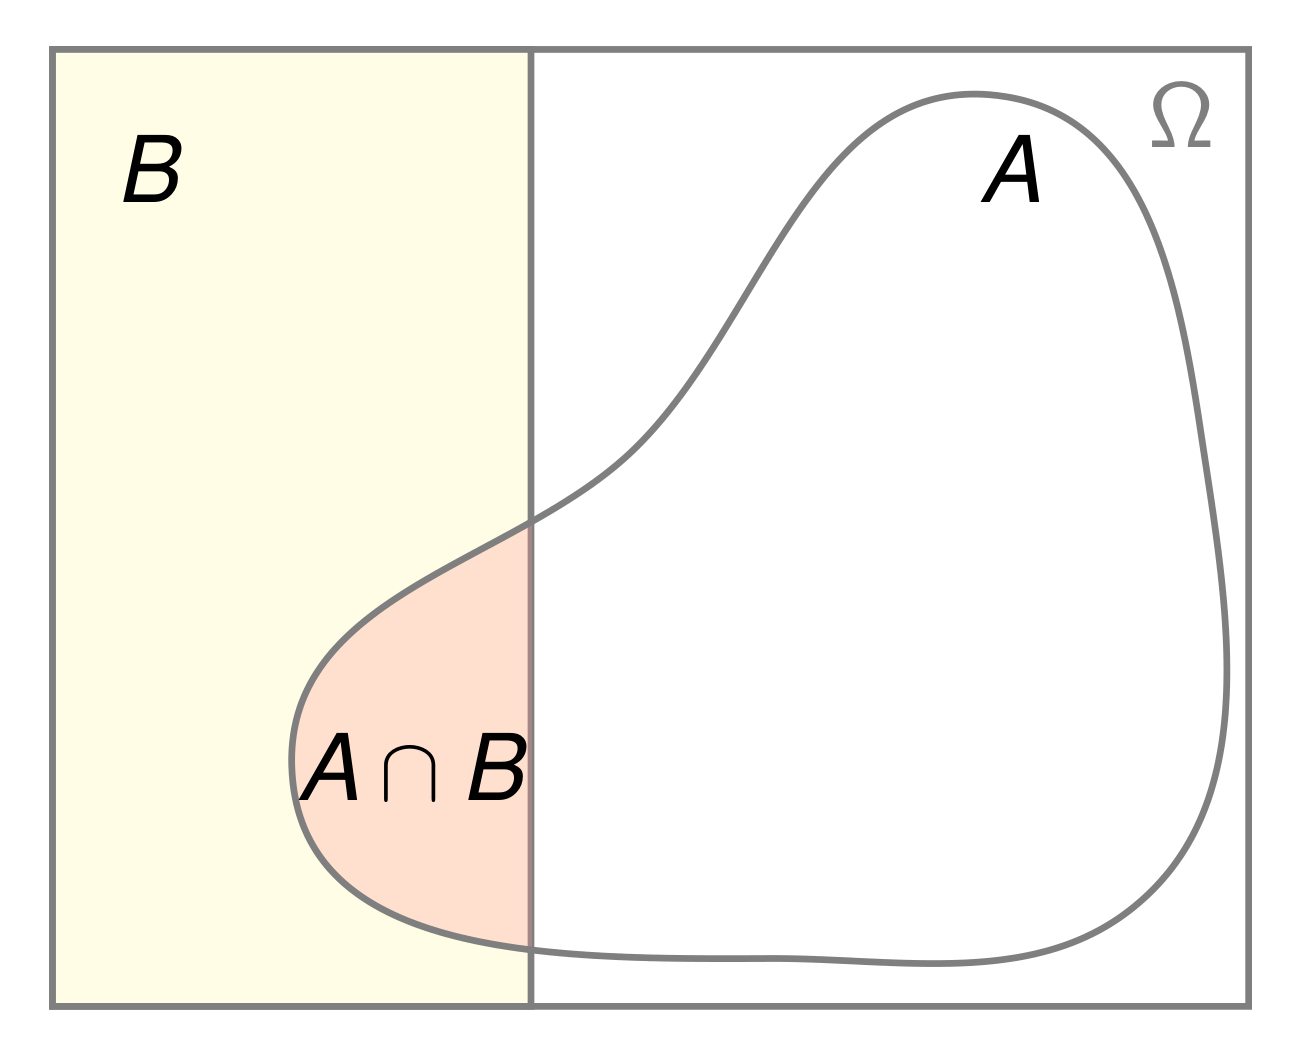
\includegraphics[width=\linewidth, keepaspectratio]{img/A_given_B}
\end{minipage}
\begin{minipage}{0.7\linewidth}
	Given that $B$ has occurred, possible outcomes must be in $B$. Thus $P(A|B)$ is the probability, that the outcome is in A.
\end{minipage}

\paragraph{Example - Coin Toss}
Let $A$ be the event of two Heads in three tosses of a fair coin. $B$ is the event that the first coin of the three tosses is a Head.
\begin{equation*}
	\Omega = \{HHH, HHT, HTH, THH, HTT, THT, TTH, TTT\}
\end{equation*}


\noindent
\begin{minipage}{\textwidth}
	\renewcommand{\arraystretch}{1.5}
	\centering
	\begin{tabularx}{\linewidth}{l X}
		$ A = \{HHT, HTH, THH\}$ & $P(A) = \frac{3}{8}$\\
		$ B = \{HHH, HHT, HTH, HTT\}$ & $P(B) = \frac{4}{8}$ \\
		$ A|B = \{HHT,HTH\} | \{HHH,HHT,HTH,HTT\}$ & $P(A|B) = \frac{2}{4}$\\
		$ B|A = \{HHT,HTH\} | \{HHT,HTH,THH\}$ & $P(B|A) = \frac{2}{3}$\\
		\multicolumn{2}{l}{$ P(A,B) = P(A)\cdot P(B|A) = P(B)\cdot P(A|B) = \frac{3}{8}\cdot\frac{2}{3}=\frac{4}{8}\cdot\frac{2}{4}=\frac{2}{8} $}\\
		\multicolumn{2}{l}{$ P(A|B) = \frac{P(B|A)\cdot P(A)}{P(B)} = \frac{\frac{2}{3}\cdot\frac{3}{8}}{\frac{4}{8}}=\frac{2}{4} $}
	\end{tabularx}
\end{minipage}

\subsection{Bayes Theorem}
\begin{equation*}
	P(A|B) = \frac{P(B|A)\cdot P(A)}{P(B)} = \frac{P(B|A)\cdot P(A)}{\sum_{i=1}^{n}P(B|A_i)\cdot P(A_i)}
\end{equation*}
if $A_i \quad i=1,...,n$ is a decomposition of $\Omega$.

In our setting with parameter or parameter vector $\theta$ and observed data $D$:

\begin{equation*}
	P(\theta|D) = \frac{\overbrace{P(D|\theta)}^{\text{likelihood}}\overbrace{P(\theta)}^{\text{prior}}}{\underbrace{P(D)}_{\text{normalizing constant}}} = \frac{P(D|\theta)P(\theta)}{\sum_{i=1}^{n}P(D|\theta_i)P(\theta_i)}\propto P(D|\theta)P(\theta)
\end{equation*}

\subsection{Approximate Bayesian Computation}
\paragraph{Rejection Algorithm} Repeat:
\begin{itemize}
	\item Sample $\theta$ from the prior distribution p($\theta$)
	\item Sample $D_i$ from the sampling distribution or generative model $p(D|\theta)$
\end{itemize}
\noindent
Collect $\theta$ if $D_i = D$. The rejection algorithm samples from the posterior distribution. If $D$ is discrete, the rejection algorithm is exact.

\vspace{1em}
\noindent
Collect $\theta$ if $\norm{D_i - D} < \epsilon$. This variant is applicable for continuous data, adjust the tolerance $\epsilon$ to trade-off between precision and efficiency.

\vspace{1em}
\noindent
Collect $\theta$ if $\abs{T(D_i ) - T(D)} < \epsilon$. Use summary (sufficient) statistic T to reduce complexity. A statistic is sufficient for a probability distribution if the sample from which it is calculated gives no additional information compared to the statistic, so you don't lose information by using $T(D)$.

\subsection{A/B Testing}
\textbf{A/B testing} is a way to compare two alternatives, typically by testing a subject's response to variant A against variant B, and determining which of the two variants is more effective.

\subsubsection{Build Simulation}

\begin{center}
	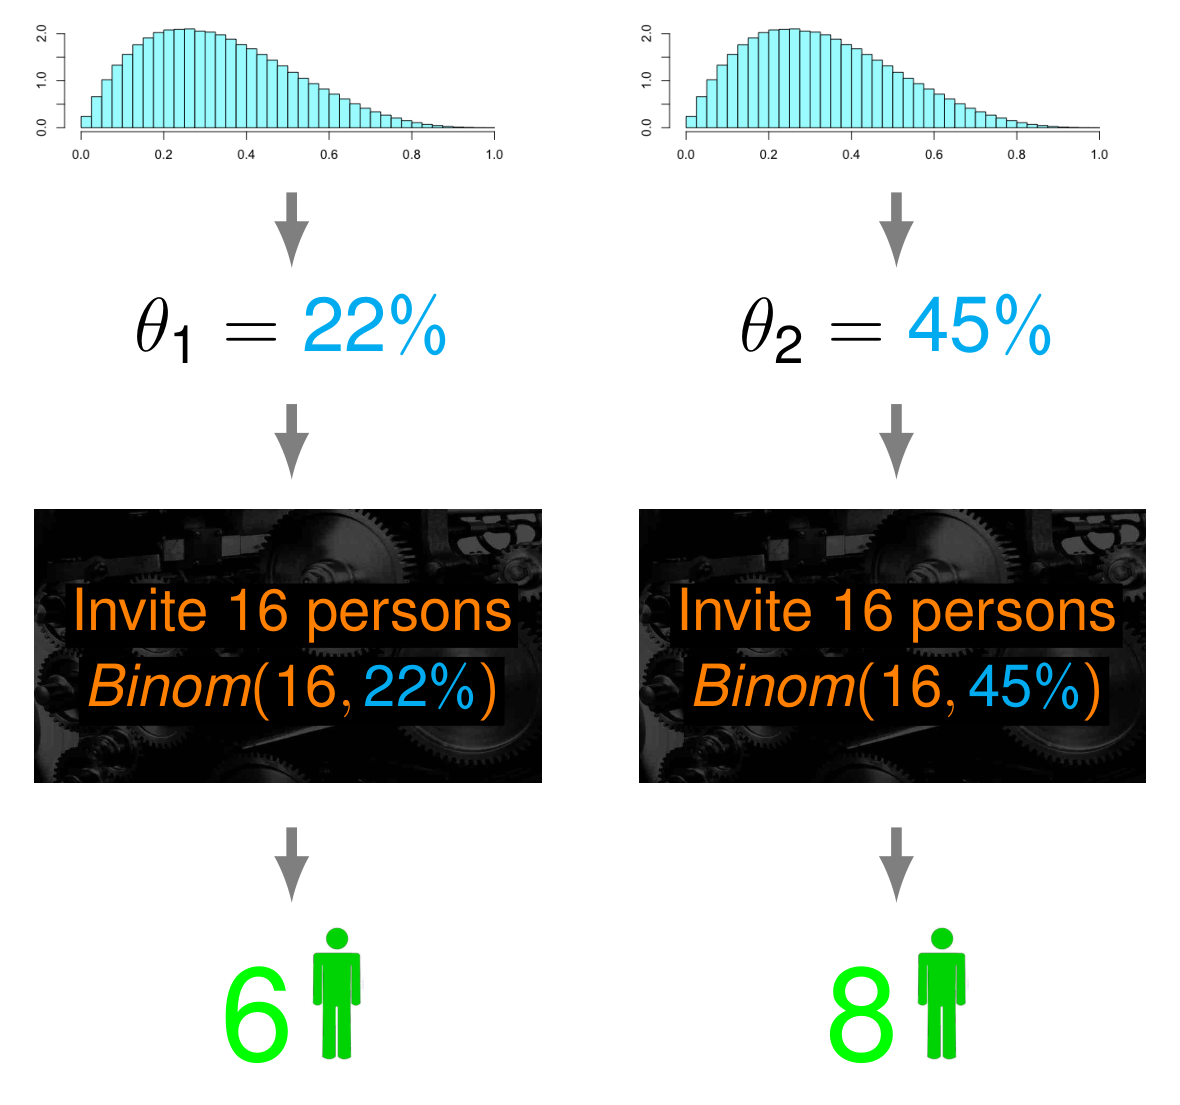
\includegraphics[width=0.5\linewidth]{img/ab_simulation_model}
\end{center}

Simulate until you observe the data (in this case 6 and 10 sign-ups). A random sample from our model consists of \textbf{four sampled parameters}: $\theta_1$ , $\theta_2$ and the number of sign-ups in method A and B. We are interested in sampled rates $\theta_1$ for method A and $\theta_2$ for method B that leads to 6 sign ups in method A and 10 sign-ups in method B.

\begin{tabularx}{\linewidth}{l l l}
	& method A & method B\\
	& $\theta_1$ & $\theta_2$\\
	1 & 28\% & 74\% \\
	2 & 31\% & 34\% \\
	3 & 41\% & 29\% \\
	4 & 26\% & 61\% \\
	$\vdots$ & $\vdots$ & $\vdots$
\end{tabularx}

These rates are a random sample from our model conditional on \textbf{6 sign-ups in method A} and \textbf{10 signups in method B} and form the posterior distribution of sign-up rates $\theta_1$ and $\theta_2$ .

\subsubsection{Evaluation}

\begin{center}
	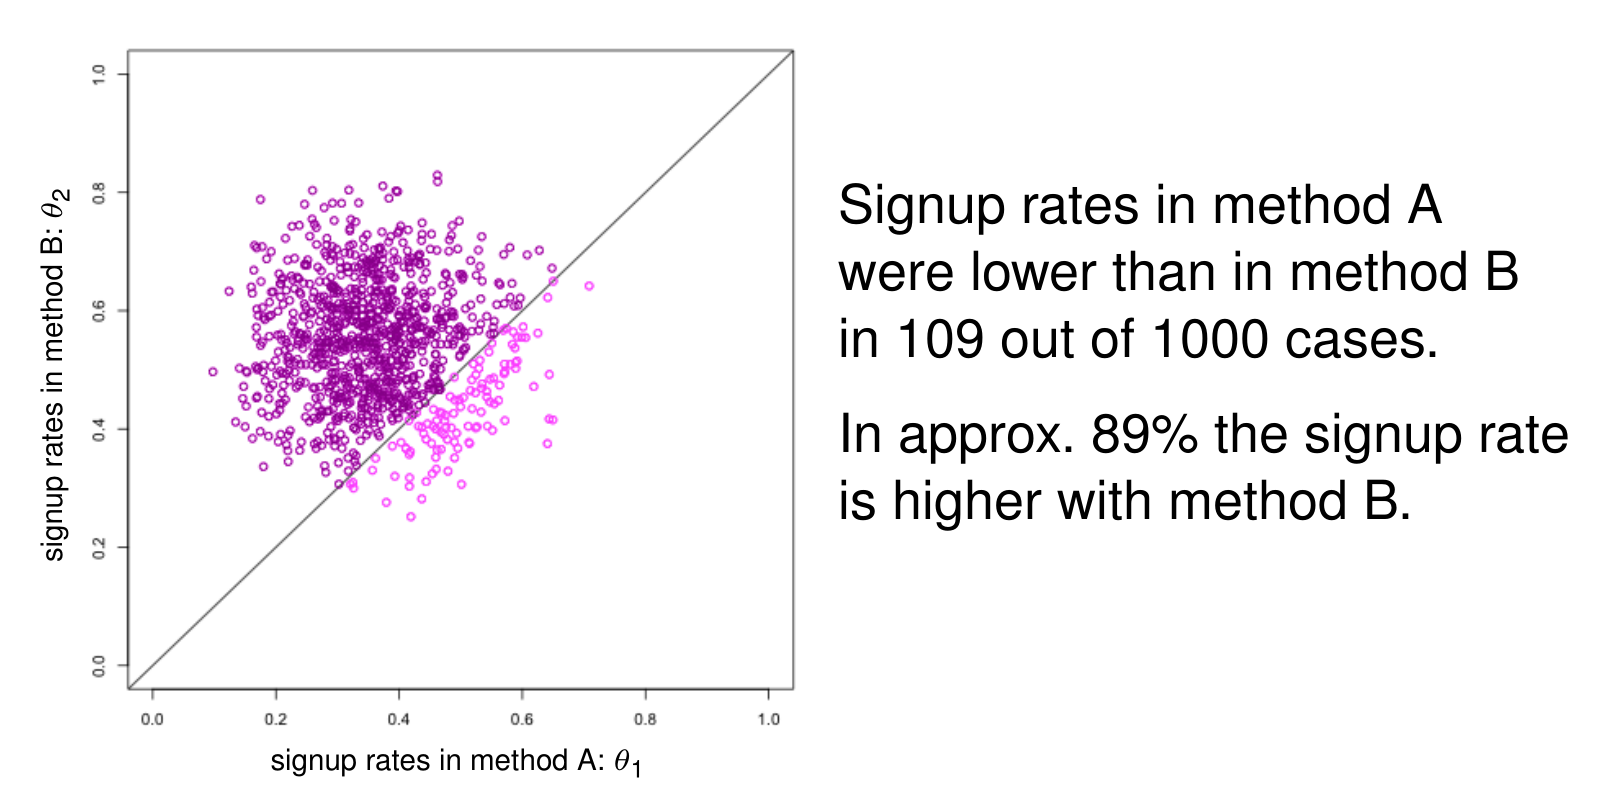
\includegraphics[width=0.6\linewidth]{img/ab_simulation_evaluation}
\end{center}
\begin{center}
	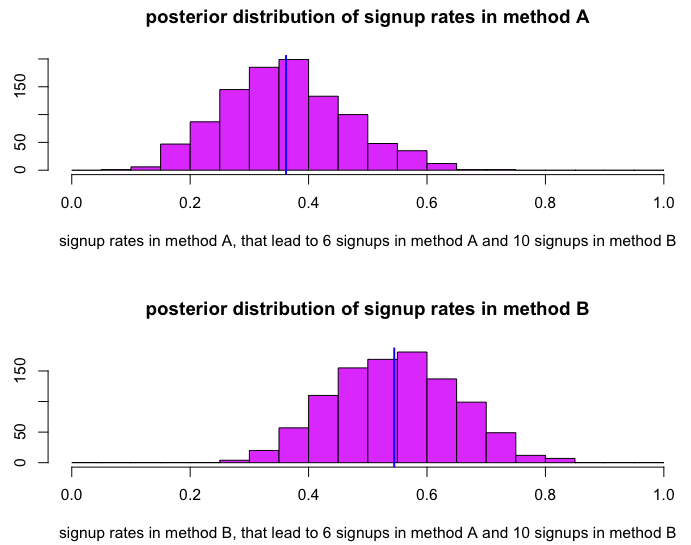
\includegraphics[width=0.6\linewidth]{img/ab_simulation_evaluation_signup}
\end{center}

\section{Exact Bayesian Analysis - Discrete Probability Models}

\subsection{Bayesian Inference}
A recap for the recipe to do Bayesian Data Analysis
\begin{itemize}
	\item Acquire Observations or Data D
	\item Formulate a model with parameters $\theta = (\theta_1, \theta_2, \theta_k)$
	\item $p(\theta)$ is the prior distribution
	\item $p(D|\theta)$ is the likelihood function, which specifies the sampling distribution of the generative model
	\item Use Bayes theorem to compute the posterior distribution
	\begin{equation*}
	p(D|\theta) = \frac{p(D|\theta)p(\theta)}{p(D)}\propto p(D|\theta)p(\theta)
	\end{equation*}
\end{itemize}

In Approximate Bayesian Computation (ABC) you don't need to calculate anything, instead you sample from the prior distribution and the likelihood function.

\subsection{Binomial Distribution}
If the \textbf{generative model is $\text{Binom}(n,\theta)$} for a given $n$, you have a one parameter family of discrete distributions. The parameter $\theta$ is often interpreted as the probability of success in $n$ trials of an experiment, the rate of failure or a certain fraction.

\subsubsection{Conjugate Prior for the Binomial Model}

If you use a \textbf{Beta distributed prior} on the parameter $\theta$ for the Binomial distribution, the resulting \textbf{posterior distribution is again a Beta distribution}. This makes the Bayesian approch simple, because you get the posterior distribution instantly. 

Thus the Beta distribution is said to be a \textbf{conjugate prior} for the parameter $\theta$ of the Binomial distribution.

Consider $\text{Binom}(n, \theta)$ as the underlying generative model. Here, the parameter $\theta$ refers to the probability of success in one trial of the experiment. When $s\leq n$ successes are observed, the likelihood of the data is given by:

\begin{equation*}
	\mathcal{L}(\theta) = P(D|\theta) = \binom{n}{s}\theta^s(1-\theta)^{n-s}
\end{equation*}

If the prior on $\theta$ is Beta distributed ($\theta \sim \text{Beta}(a,b)$), then the posterior distribution is given by 
\begin{equation*}
	\theta|D \sim \text{Beta}(a + s, b + n - s)
\end{equation*}

\subsubsection{Beta Update for the Binomial Model}
We observe $k$ experiments, all with the same unknown success probability $\theta$. In experiment $i$ we count $s_i$ out of $n_i$ successes.

If the prior distribution on $\theta$ is $\text{Beta}(a,b)$, then the posterior distribution on $\theta$ is given by

\begin{equation*}
	p(\theta|D) \sim \text{Beta}\left(a+\sum_{i=1}^{k}s_i, b + \sum_{i=1}^{k} (n_i - s_i)\right)
\end{equation*}

This can be thought of as the collection of successive information by repeating experiments and updating the posterior distribution of $\theta$.

\begin{minted}{R}
# 6 sign-ups out of 16 candidates, 6 successes, 10 failures
curve(dbeta(x,1+6,1+10), col=magenta", lwd=3)
postMean = 7/(7+11)
[1] 0.3888889
qbeta(c(0.05,0.95),1+6,1+10)
[1] 5% 95%
[2] 0.2119082 0.5802946
\end{minted}

\subsubsection{Example Machine Parts}
Machine A has a daily capacity of producing 223 articles and machine B can produce 219 articles. In two test runs there were randomly occuring manufaction errors leading to 14 and 18 (each out of 223) insufficient articles from machine A and 6 and 10 (each out of 219) insufficient articles from machine B.

Calculate the posterior distribution for the failure rate $\phi_A$ of machine A and the failure rate $\phi_B$ of machine B when you assume a $\text{Beta}(2,25)$-prior on failure rates.

Simulate: What’s the probability that machine A produces more acceptable articles than machine B in a day?

\begin{minted}{R}
curve(dbeta(x,2,25),0,.2)
curve(dbeta(x,2+14+18,25+223-14+223-18),0,.2,add=TRUE)
curve(dbeta(x,2+6+10,25+219-6+219-10),0,.2,add=TRUE)
ma = rbinom(10000,223,1-rbeta(10000,2+32,25+414))
mb = rbinom(10000,219,1-rbeta(10000,2+16,25+422))
sum(ma>mb)/10000
[1] 0.2442
\end{minted}

\subsection{Geometric Distribution}
The geometric distribution takes values in $\mathbb{N}_0 = 0,1,2,3,...$ . It represents the number of failures in a sequence of Bernoulli trials before a success occurs.

The probability of a geometric distributed random variable $X \sim \text{Geom}(\theta)$ with success probability $\theta$ for $n \in \mathbb{N}_0$ is:
\begin{equation*}
	P(X=n|\theta) = \theta (1 - \theta)^n
\end{equation*}

\noindent
$\mathbb{E}(X)=\frac{1-\theta}{\theta}$, $\text{Var}(X) = \frac{1-\theta}{\theta^2}$

\subsubsection{Conjugate Prior for the Geometric Model}
Let $X\sim \text{Geom}(\theta)$. We observe $x$ failures before success and want to infer the success probability $\theta$.

With a $\text{Beta}(a,b)$ distributed prior on $\theta$, the posterior distribution is
\begin{equation*}
	\text{Beta}(a+1, b+x)
\end{equation*}

Considering $n$ observation with outcomes $x_1, x_2, ... ,x_n$, that is $x_i$ failures in an experiment $i$ before a success occurs. With a $\text{Beta}(a,b)$ distributed prior on $\theta$, the posterior distribution is

\begin{equation*}
	\text{Beta}(a+n, b+\sum_{i=1}^{n}x_i)
\end{equation*}

\subsection{Possion Distribution}
The Poisson distribution counts the number of rare events in a fixed interval of time or space if these events occur randomly and independent from each other with a constant rate.

The distribution takes values in $\mathbb{N}_0 = 0,1,2,3,...$

The density of a Poisson distributed random variable $X \sim \text{Pois}(\lambda)$ on $n \in \mathbb{N}_0$ with parameter $\lambda > 0$ is given by:

\begin{equation*}
	p(X) = p(X=n|\lambda) = \frac{\lambda^n}{n!}e^{-\lambda}
\end{equation*}
\noindent
$\mathbb{E}(X) = \lambda$, $\text{Var}(X) = \lambda$

\begin{center}
	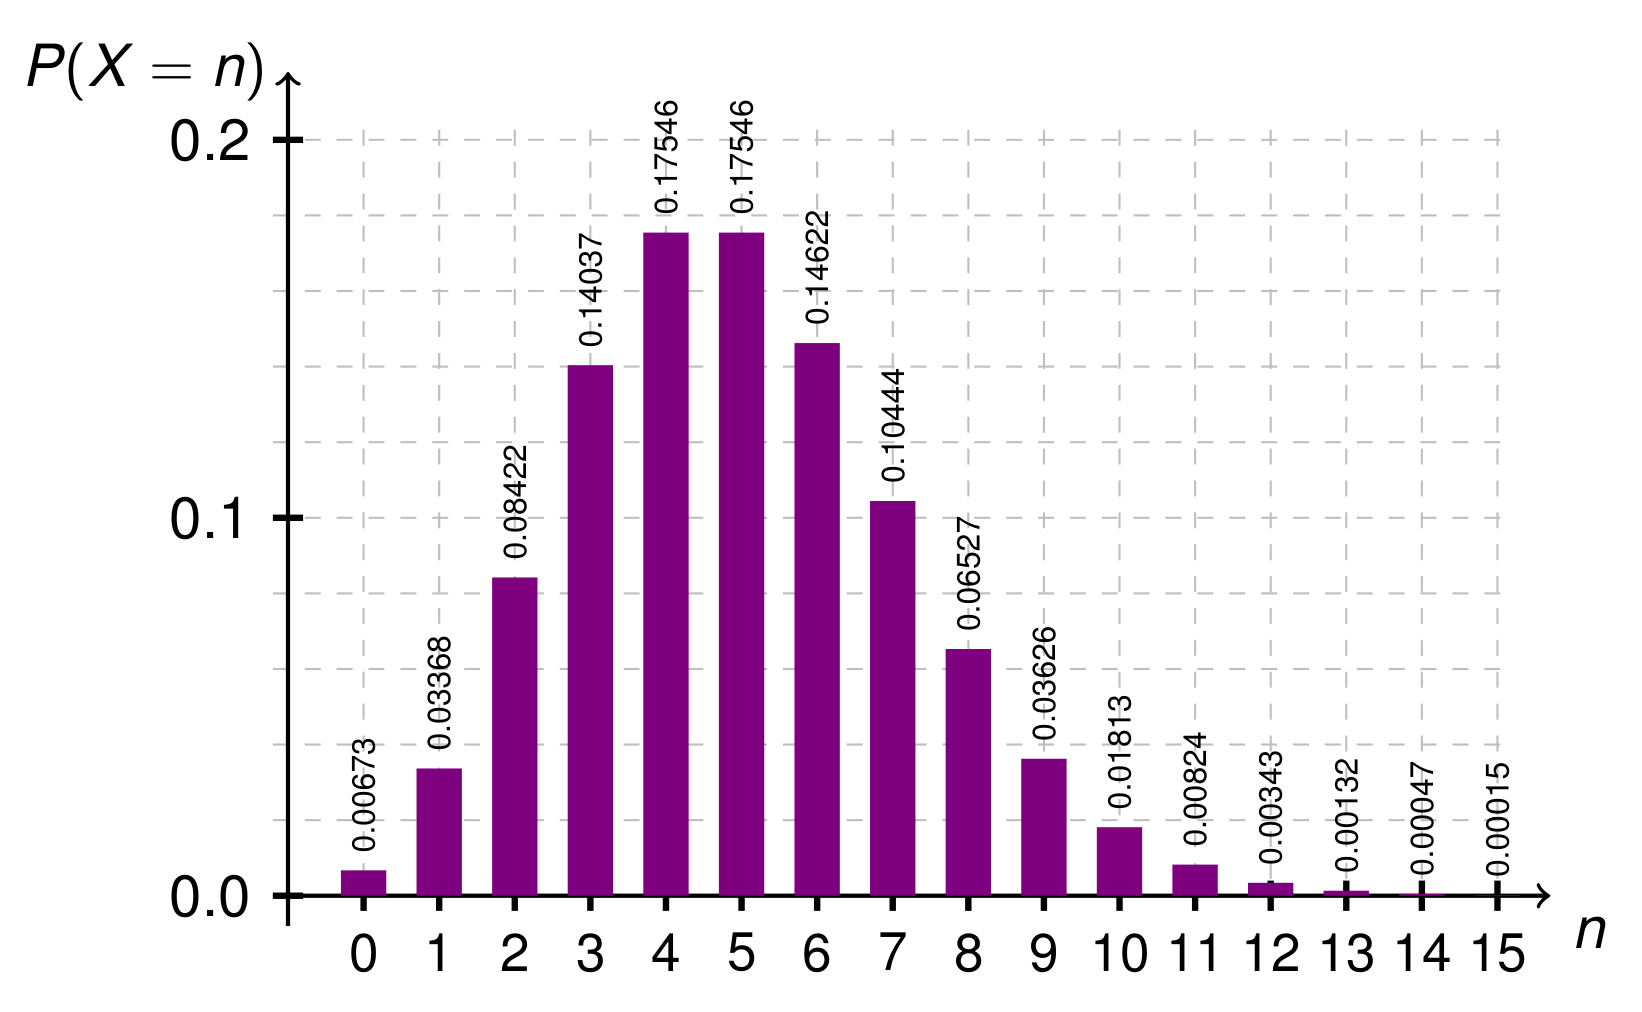
\includegraphics[width=0.7\linewidth]{img/poisson_distribution_lambda5}
\end{center}

The Poisson distribution is used to model intervals in a space or over time. For example
\begin{itemize}
	\item $X$ equal the number of typos (interval) on a printed page (space)
	\item $X$ equal the number of cars (interval) passing a certain route in one hour (time)
	\item $X$ equal the number of Alaskan salmon (interval) caught in a squid drift net (space)
	\item $X$ equal the number of students (interval) arriving during office hours
\end{itemize}

\subsubsection{Conjugate Prior for the Poisson Model}
Let $X\sim \text{Pois}(\lambda)$. That is, we expect on average $\lambda$ events per observation period. 

Consider $x$ events have been observed in a given period. With a gamma prior, $\lambda \sim \text{Gamma}(a,b)$, the posterior distribution is
\begin{equation*}
	\text{Gamma}(a + x, b + 1)
\end{equation*}

If $n$ periods with $x_i, i=1...n$ events have been observed and a
$\text{Gamma}(a,b)$ prior on $\lambda$ is assumed, the resulting posterior for $\lambda$ is given by
\begin{equation*}
	\text{Gamma}(a+\sum_{i=1}^{n}x_i, b+n)
\end{equation*}

\subsection{Gamma Distribution}
A $\text{Gamma}(a,b)$ distributed random variable has values in $\mathbb{R}_0^+$.

The density of a $\text{Gamma}(a,b)$ distributed random variable $X$, with shape parameter $a$ and rate parameter $b$ is given by
\begin{equation*}
	p(x) = p(x|a,b) = \frac{b^a}{\Gamma(a)}x^{a-1}e^{-b\cdot x}
\end{equation*}
\noindent
$\mathbb{E}(X)=\frac{a}{b}$, $\text{Var}(X) = \frac{a}{b^2}$, $\text{Mode}(X) = \frac{a-1}{b}\text{ for }a\geq 1$
\begin{minted}{R}
	curve(dgamma(x,100,10),0,20,1000)
\end{minted}

\subsubsection{Example}
You recorded the counts of new customers on a daily basis for 16 days: \{2, 3, 8, 10, 4, 5, 8, 7, 2, 12, 4, 3, 7, 6, 4, 11\}.
The data can be assumed to be Poisson distributed with unknown but fixed parameter $\lambda$. 

The prior on the parameter $\lambda$ is $\text{Gamma}(5,1)$. Calculate a 90\% credible interval for $\lambda$. Whats the probability, that you have at least 5 new customers per day on average?

\begin{minted}{R}
hist(rgamma(10000,5,1))
curve(dgamma(x,5,1),0,10)
sum(c(2, 3, 8, 10, 4, 5, 8, 7, 2, 12, 4, 3, 7, 6, 4, 11))
curve(dgamma(x,5+96,1+16),0,10,add=T)
quantile(rgamma(10000,5+96,1+16),c(.05,.95))
qgamma(c(.05,.95),5+96,1+16)
1 - pgamma(5,5+96,1+16)
\end{minted}

\subsection{Hypergeometric Distribution}
The \textbf{Hypergeometric Distribution} with parameters $n$, $N$ and $M$ takes values in $0,1,2,...,\min{n,M}$. It represents the number of $m$ successes in $n$ draws \textbf{without replacement} from a set of size $N$, that contains exactly $M$ objects with a certain feature.

The probability of a Hypergeometric distributed random variable $X \sim \text{HyperGeo}(n,N,M)$ for $m \in \mathbb{N}_0$ is
\begin{equation*}
	p(X=m|n,N,M) = \frac{\binom{M}{m}\binom{N-M}{n-m}}{\binom{N}{n}}
\end{equation*}
\noindent
$\mathbb{E}(X)=n\cdot\frac{M}{N}$, $\text{Var}(X) = n\cdot\frac{M}{N}\frac{N-M}{N}\frac{N-n}{N-1}$

\begin{center}
	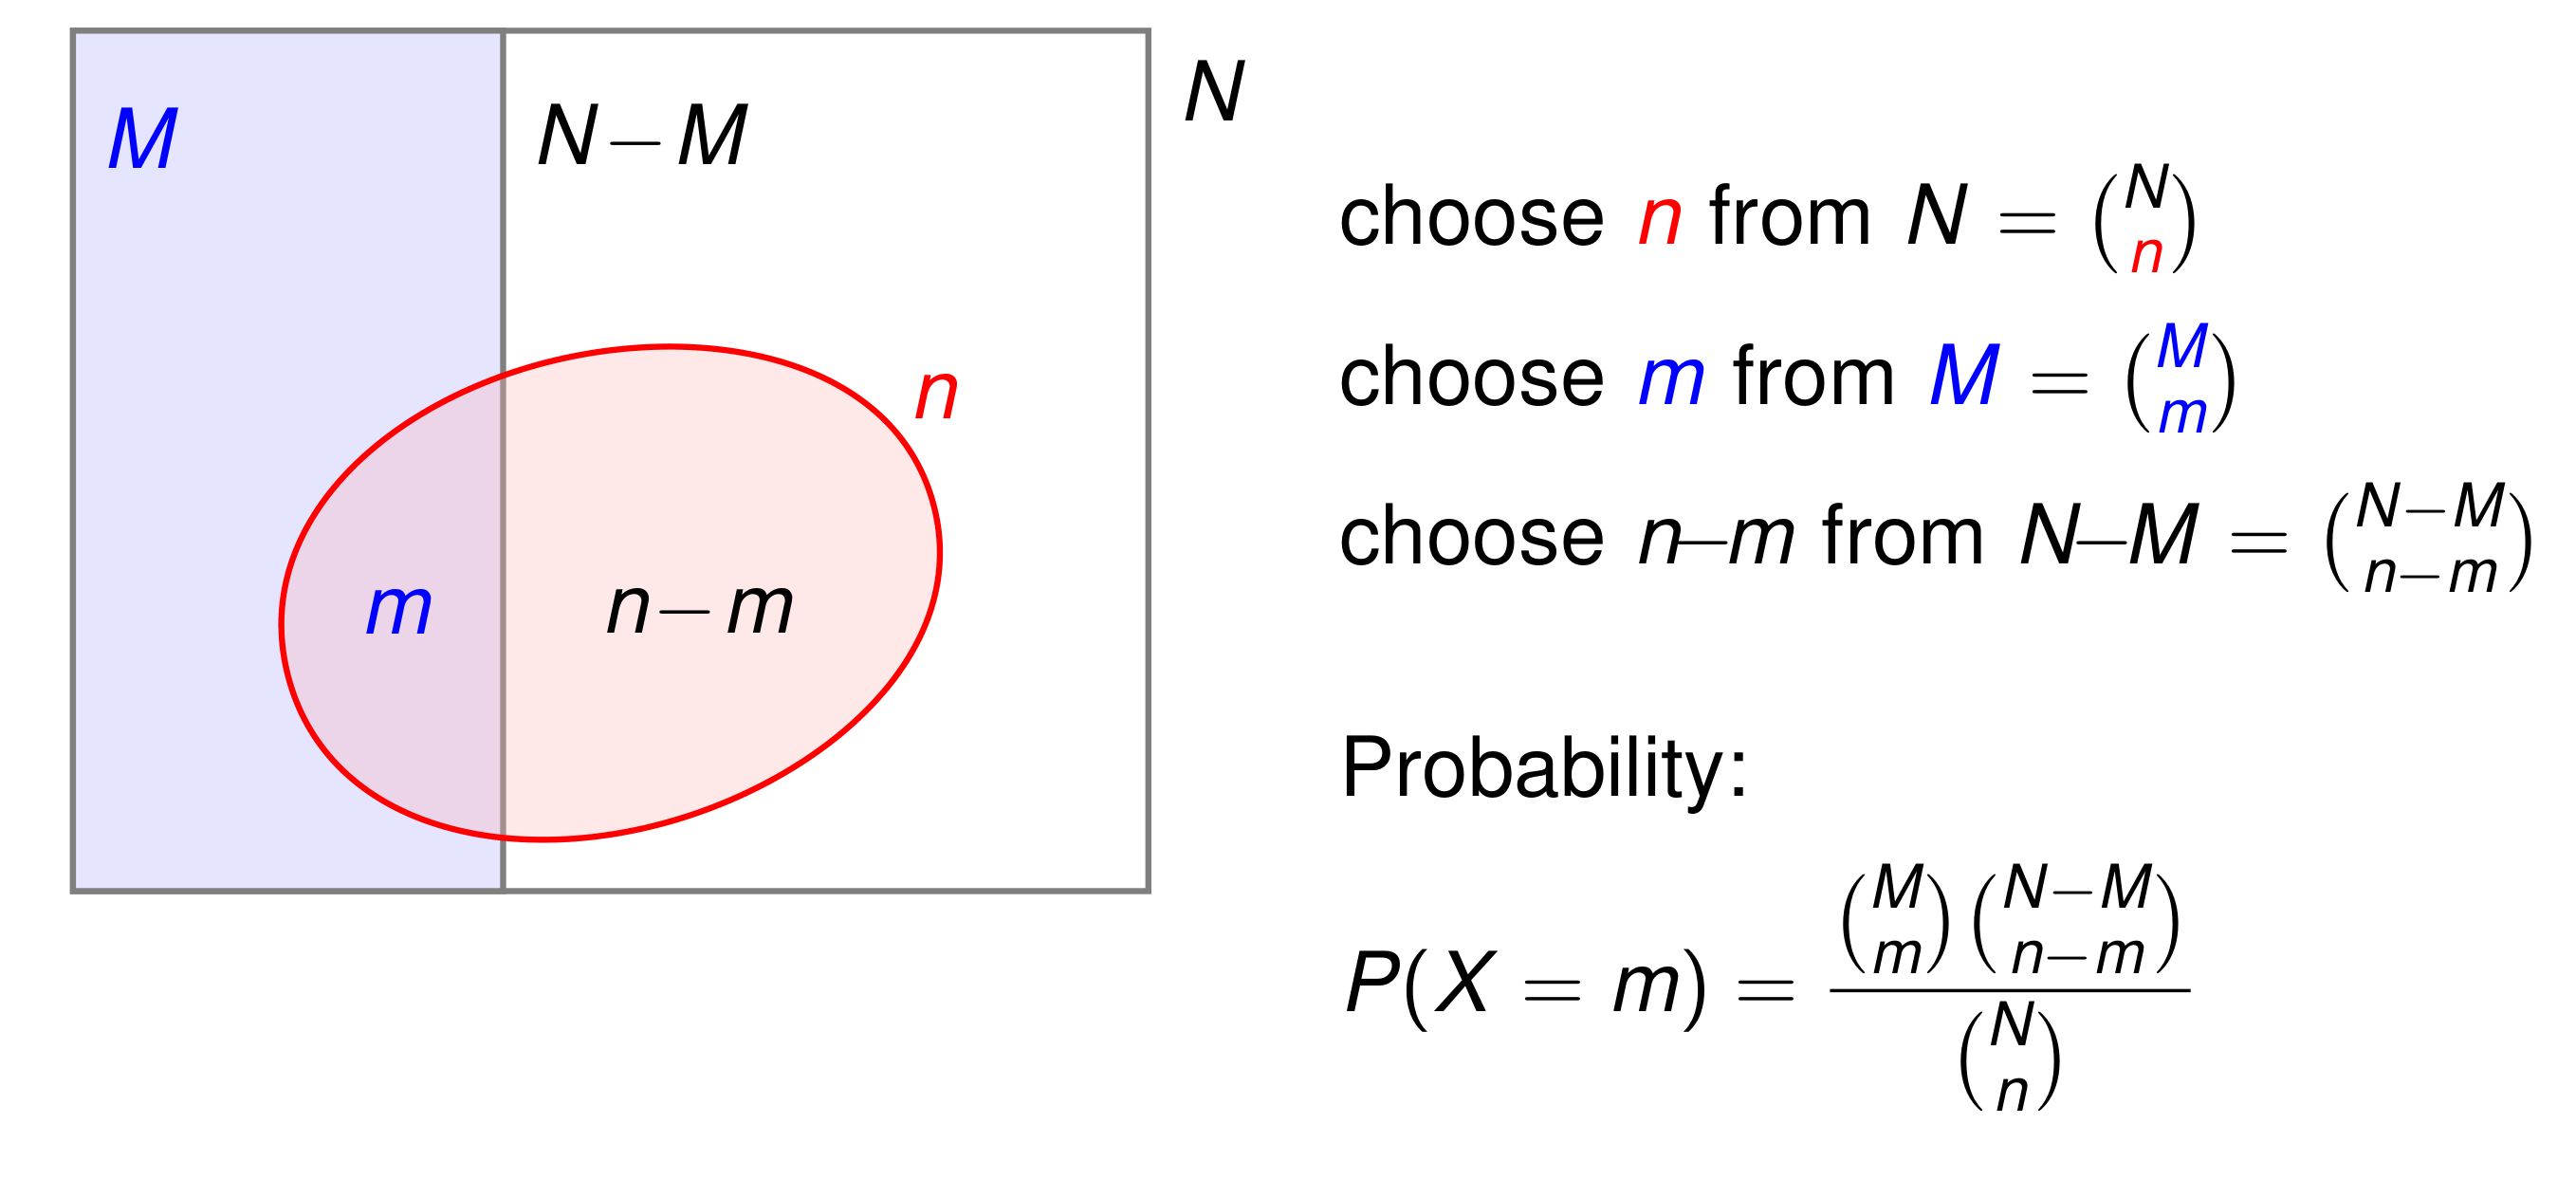
\includegraphics[width=0.7\linewidth]{img/hypergeometric_ditribution_derivation}
\end{center}

\subsubsection{Conjugate Prior for the Hypergeometric Model}
In the Hypergeometric model the total number of objects $N$ and the number of draws $n$ are given. The parameter you are interested in is $M$, that is you are uncertain about the number of objects with a certain feature. You observe a sample with $m$ objects out of $n$ with a certain feature.

With a Beta-binomial prior on $M$, that is $M \sim \text{BetaBin}(N,a,b)$ the posterior distribution of $M$ is
\begin{equation*}
	M - m \sim \text{BetaBin}(N - n,a + m,b + n - m)
\end{equation*}

where $m$ out of $n$ sampled objects (without replacement) have a given feature.

\subsection{Beta-Binomial Distribution}
The Beta-binomial distribution is a Binomial distribution with $N$ trials in which the probabilities of success are randomly drawn
 from a $\text{Beta}(a,b)$ distribution.

A $\text{BetaBinom}(N,a,b)$ distributed random variable has values $\{0,1,2,...,N\}$. With $a,b>0$ and $N\in\mathbb{N}_0$ the density is given by

\begin{align*}
	p(x) = p(x|N,a,b) &= \binom{N}{x}\frac{\text{Beta}(a+x,b+N-x)}{\text{Beta}(a,b)}\\
	&= \binom{N}{x}\frac{\Gamma(a+b)\Gamma(a+x)\Gamma(b+N-x)}{\Gamma(a)\Gamma(b)\Gamma(a+b+N)}
\end{align*}
\noindent
$\mathbb{E}(X)=N\cdot\frac{a}{a+b}$, $\text{Var}(X) = N\cdot\frac{a\cdot b}{(a+b)^2}\frac{(a+b+N)}{(a+b+1)}$

Use the R-package \mintinline{R}{rmutil} to get the density, quantiles and to simulate from a Beta-binomial distributed random variable.
\begin{minted}{R}
install.packages("rmutil")
library("rmutil")
\end{minted}

The parametrisation in this package slightly differs from the definition above:
\begin{align*}
	p(x) = p(x|N,a,b) &= \binom{N}{x}\frac{\text{Beta}(x+sm,N-x+s(1-m))}{\text{Beta}(sm,s(1-m))}\\
	M &= \frac{a}{a+b}\\
	s &= a+b\\
	a &=sm\\
	b &= s(1-m)
\end{align*}

\section{Exact Bayesian Analysis - Exponential Models}
The Exponential distribution takes values in $\mathbb{R}_0^+$ representing the waiting time until the occurrence of an event. It can be used to model the failure rate of technical components.

The density of an exponentially distributed random variabe $X \sim \text{Exp}(\lambda)$ for $x\in\mathbb{R}_0^+$ with the rate parameter $\lambda>0$ is given by
\begin{equation*}
	p(x) = p(x|\lambda) = \lambda e^{-\lambda x}
\end{equation*}
\noindent
$\mathbb{E}(X) = \frac{1}{\lambda}$, $\text{Var}(X) = \frac{1}{\lambda^2}$

\begin{minted}{R}
curve(dexp(x,2),0,5)
curve(dexp(x,1),0,5,add=T)
curve(dexp(x,.5),0,5,add=T)
\end{minted}

\begin{center}
	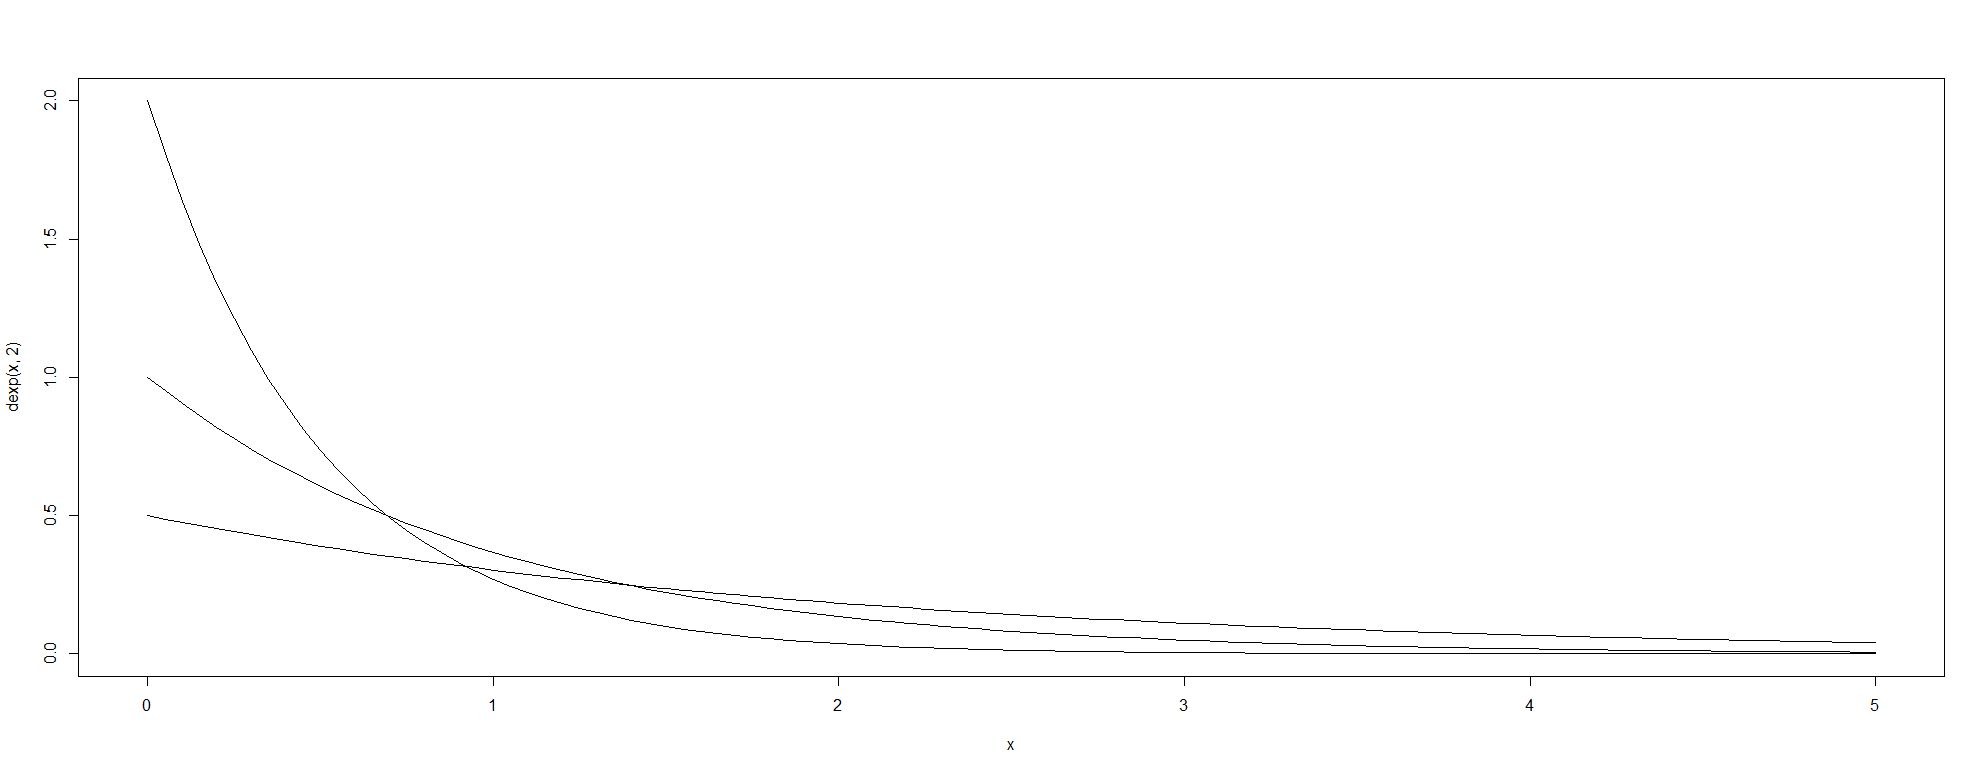
\includegraphics[width=0.8\linewidth]{img/exponential_distribution_curves}
\end{center}

Let $X \sim \text{Exp}(\lambda)$, that is we expect to observe the time $\frac{1}{\lambda}$ between two events on average. Consider we observe the time $t$ between evenets.

With a $\text{Gamma}(a,b)$ prior on $\lambda$ ($\lambda \sim \text{Gamma}(a,b)$), the posterior distribution on the failure rate $\lambda$ is
\begin{equation*}
	\text{Gamma}(a+1,b+t)
\end{equation*}

If we observe $n$ time intervals $t_i\quad i=1..n$ between failures in components and assume a $\text{Gamma}(a,b)$ prior on $\lambda$, then the resulting posterior on $\lambda$ is
\begin{equation*}
	\text{Gamma}(a+n,b+\sum_{i=1}^{n} t_i)
\end{equation*}

\subsubsection{Example}

There are usually between 6 and 14 failures of remote computers per day in a certain computing center. The following list contains 16 waiting times in minutes between consecutive failures: 290, 60, 120, 30, 30, 180, 830, 40, 320, 60, 90, 450, 800, 620, 30 and 90. The sum is 4040 minutes.
\begin{enumerate}
	\item Model an appropriate prior distribution.
	\item What's the probability, that the waiting time to the next failure is less than 30 minutes?
	\item How many events with two (or more) failures within 30 minutes do you expect per year?
	\item Calculate the MAP estimate for the parameter $\lambda$.
	\item What's the distribution on the number of failures per day?
\end{enumerate}

\begin{minted}{R}
# Find apropriate prior - 6 and 14 failures per 24*60 minutes
6/(24*60)
[1] 0.004166667
10/(24*60)
[1] 0.006944444
14/(24*60)
[1] 0.009722222
hist(rgamma(10000,7,1000))
\end{minted}

\begin{minted}{R}
curve(dgamma(x,7+16,1000+4040),0,0.01)
abline(v=c(0.0069, 16/4040))
times = rexp(1000000,rgamma(1000000,7+16,1000+4040))
hist(times,breaks=50)
sum(times<30)/1000000
[1] 0.127653
\end{minted}

\begin{minted}{R}
# Simulate and count events with less than 30min
nEvents = sum(times<30)
nYears = sum(times)/60/24/365
nEvents/nYears
[1] 292.4468
\end{minted}

\begin{minted}{R}
# MAP estimate
curve(dgamma(x,7+16,1000+4040),0,0.01)
\end{minted}

\paragraph{MAP estimate}
\begin{equation*}
	\frac{\alpha-1}{\beta} = \frac{22}{5040} = 0.0044
\end{equation*}

\paragraph{Distribution on the number of failures} Poisson Distribution

\subsection{Properties of the Exponential Distribution}

The exponential distribution is \textbf{memoryless}. The waiting time until a certain event occurs, does not depend on how much time has elapsed already. The probability for the time to the next event stays the same and is independent when you start the observation.

Consider you have $n$ \textbf{identical components}. Each component has the same failure rate $\lambda$. Then, the failure rate for observing a failure in one of the n components is $n\lambda$.

\subsection{Gaussian Model}

The Gaussian or Normal distribution is very common in statistics and takes values in $\mathbb{R}$. The central limit theorem shows that under weak conditions i.i.d. observations converge to a normal distribution.

The density of the Gaussian distributed random variable $X \sim \mathcal{N}(\mu,\sigma^2)$ for $x\in\mathbb{R}$ with mean $\mu$ and standard deviation $\sigma$ is given by
\begin{equation*}
	p(x) = p(x|\mu,\sigma) = \frac{1}{\sqrt{2\pi}\sigma}e^{\frac{(x-\mu)^2}{2\sigma^2}}
\end{equation*}
\noindent
$\mathbb{E}(X) = \text{Mode}(X) = \mu$, $\text{Var}(X)=\sigma^2$ 

\begin{center}
	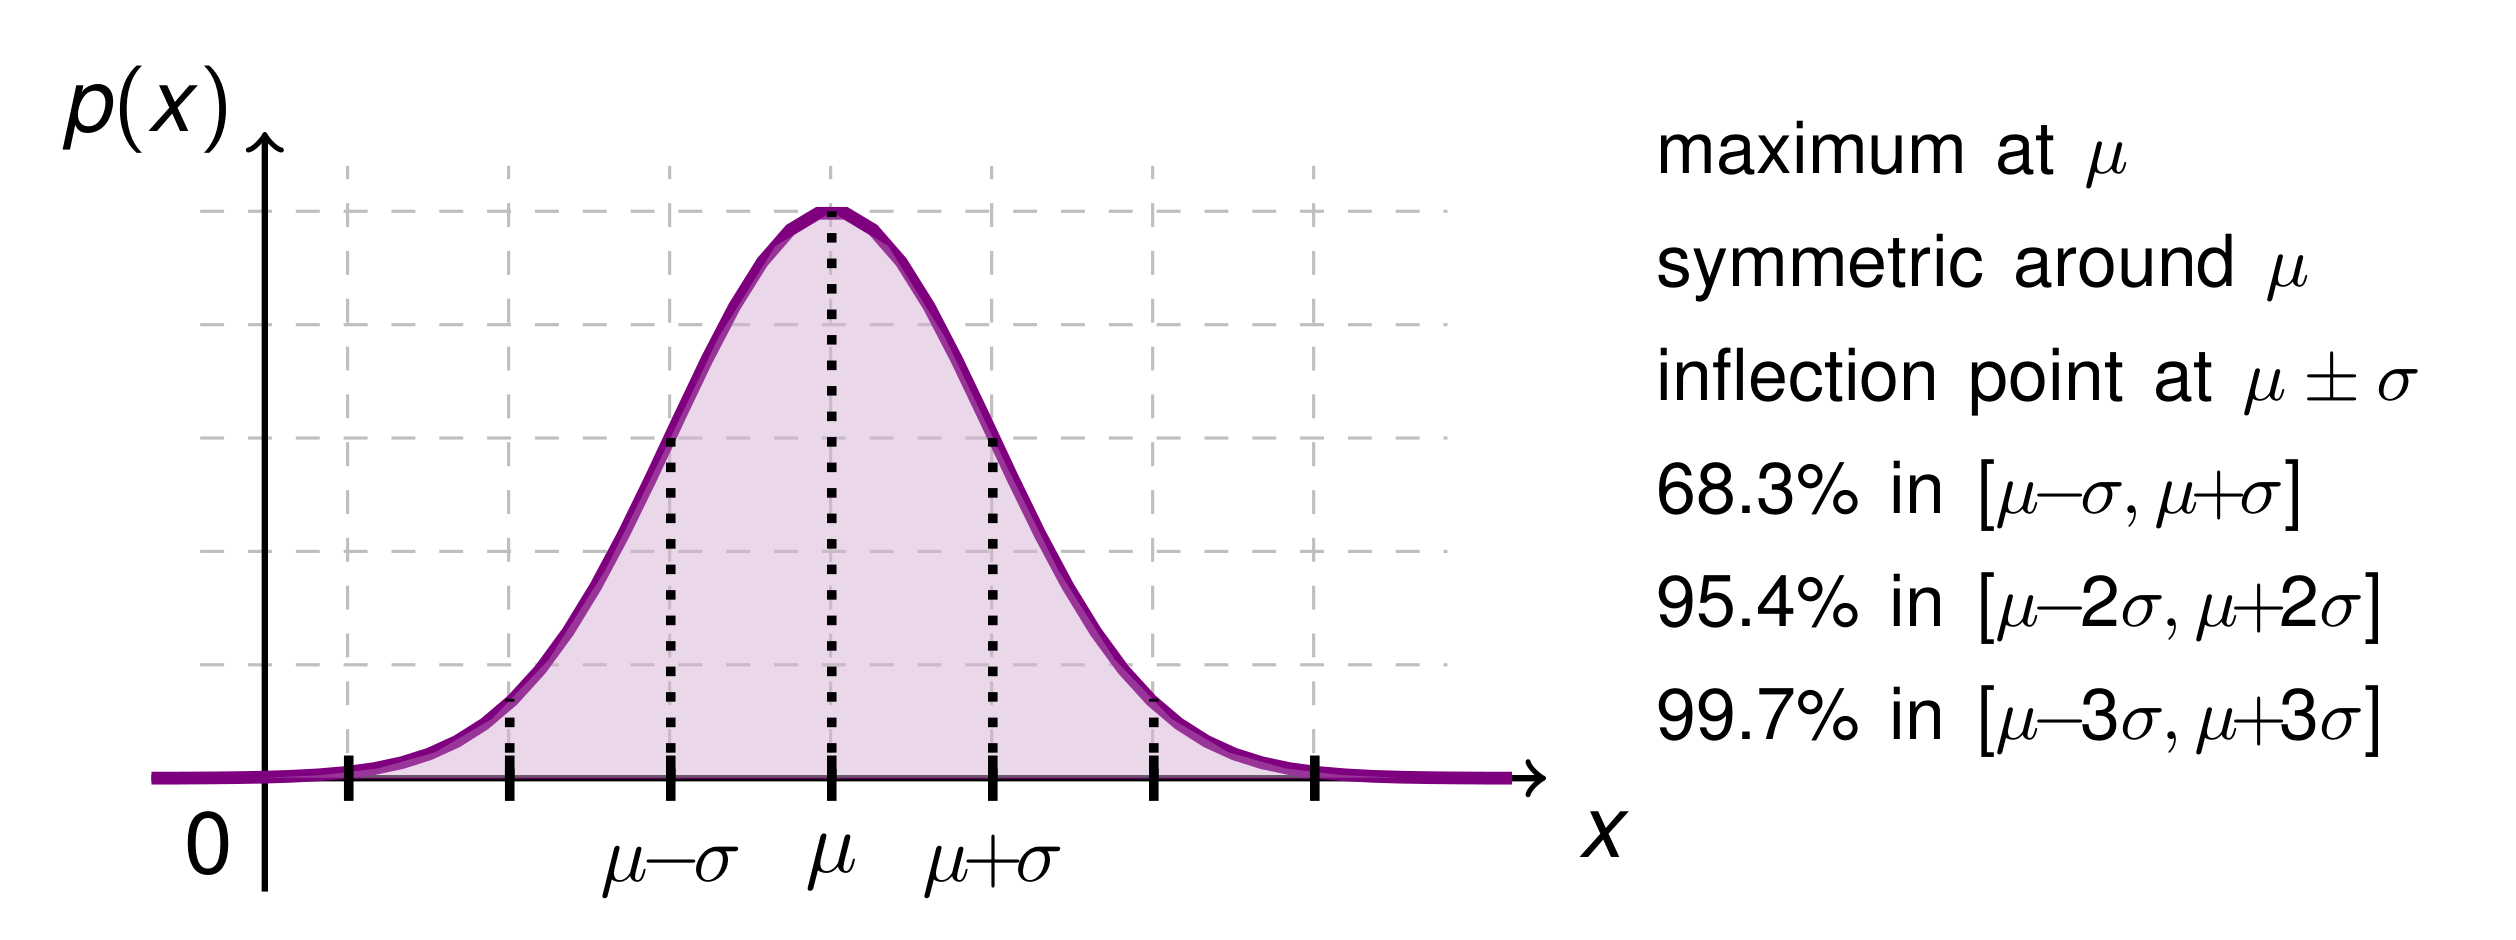
\includegraphics[width=0.7\linewidth]{img/gaussian_distribution_density}
\end{center}

\subsubsection{Conjugate Prior for $\mu$ of the Gaussian Model}
If the posterior distributions $p(\theta | x)$ are in the same probability distribution family as the prior probability distribution $p(\theta)$, the prior and posterior are then called conjugate distributions, and the prior is called a conjugate prior for the likelihood function.

Let $X \sim \text{Norm}(\mu,\sigma^2)$ with a fixed standard deviation $\sigma$. Consider, we observe a sample $x_1 ,x_2 ,...,x_n$ from $X$. With a $\text{Norm}(m,s^2)$ prior on $\mu$, the posterior distribution of $\mu$ is
\begin{equation*}
	\text{Norm}\left(\frac{ \frac{m}{s^2} + \frac{ \sum_{i=1}^{n} }{ \sigma^2 } }{ \frac{1}{s^2} + \frac{n}{\sigma^2} } , \frac{1}{\frac{1}{s^2} + \frac{n}{\sigma^2}}\right)
\end{equation*}

Thus, the posterior distribution of $\mu$ is Gaussian with mean $\frac{ \frac{m}{s^2} + \frac{ \sum_{i=1}^{n} }{ \sigma^2 } }{ \frac{1}{s^2} + \frac{n}{\sigma^2} }$ and standard deviation $\sqrt{\frac{1}{s^2} + \frac{n}{\sigma^2}}$.

\subsubsection{Conjugate Prior for $\sigma$ of the Gaussian Model}
Let $X \sim \text{Norm}(\mu,\sigma^2)$ with a fixed standard deviation $\sigma$. Consider, we observe a sample $x_1 ,x_2 ,...,x_n$ from $X$. With a $\text{Gamma}(a,b)$ prior on the precision $\tau$, where $\tau = \frac{1}{\sigma^2}$, the posterior distribution of $\tau$ is
\begin{equation*}
	\text{Gamma}\left( a+\frac{n}{2}, b + \frac{\sum_{i=1}^{n} (x_i - \mu)^2 }{2} \right)
\end{equation*}

\section{Monte Carlo Markov Chain Methods}

The aim of a Bayesian analysis is to quantify the posterior distribution of unknown parameters, to retain uncertainty and assess regions of plausible parameters values. There are three approaches to look at:
\begin{itemize}
	\item \textbf{Approximate Bayesian Computation}\quad Specifying a full probabilistc model, without calculating the likelihood function of the model. Simulate from the model and condition on observed data. Too slow for most applications.
	\item \textbf{Bayesian Analysis}\quad Use a conjugate prior to calculate the posterior. Update the parameters of the posterior. Fast but not possible with complex models.
	\item \textbf{Markov Chain Monte Carlo}\quad method to sample from an arbitrary posterior distribution, without fully describing the posterior’s probability density.
\end{itemize}

Monte Carlo is the idea of using independent, identically distributed samples $X_1 , ... , X_n$ of a random generator with density $p$ to approximate expectations
\begingroup
\renewcommand*{\arraystretch}{1.5}
\begin{equation*}
	\mu = \mathbb{E}_p(g(X)) = \left\{ \begin{matrix}
		\int_{\mathbb{R}} x\cdot g(x)p(x) dx & \text{continuous density}\\
		\sum_{i} g(x_i) \cdot p_i &\text{discrete probabilities}
	\end{matrix} \right.
\end{equation*}
\endgroup
\noindent
by sample averages 
\begin{align*}
	\widehat{\mu}&=\frac{1}{n}\sum_{i=1}^{n}g(X_i)\\
	\text{Var}(\widehat{\mu}) &= \frac{1}{n-1}\sum_{i=1}^{n}(g(X_i)-\widehat{\mu})^2
\end{align*}

\subsection{Markov Chains}
Markov chain Monte Carlo is the idea of getting samples $X_1 , ... , X_n$ from a distribution $\pi$ with the help of a Markov chain to approximate expectations
\begin{equation*}
	\mu = \mathbb{E}_\pi (g(X))
\end{equation*}
by sample averages
\begin{equation*}
	\widehat{\mu}=\frac{1}{n}\sum_{i=1}^{n}g(X_i)
\end{equation*}
where $\pi$ is the equilibrium distribution, also called invariant or stationary distribution, of the Markov chain. The Monte Carlo Markov Chain is used to build a random sampler to be able to sample from a desired distribution $\pi$.

\begin{figure}[H]
	\centering
	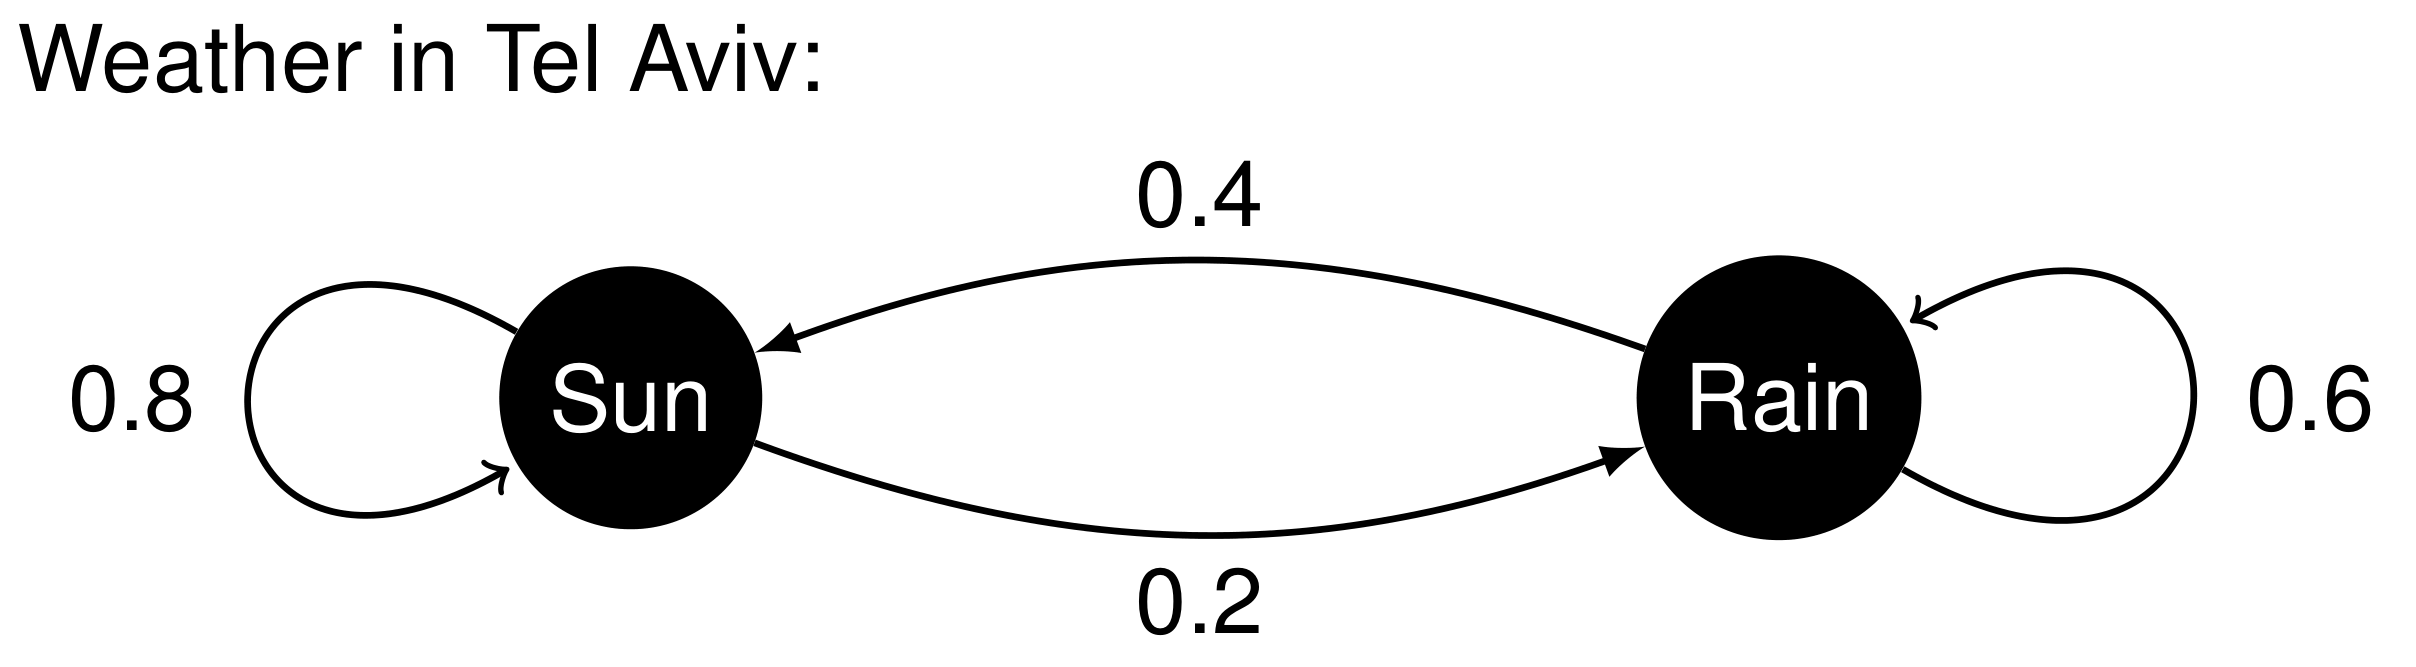
\includegraphics[width=0.6\linewidth]{img/markov_chain_example}
	\caption{Example for a Markov chain, here the changes in weather in Tel Aviv}
	\label{fig:markovchainexample}
\end{figure}

\noindent
State space $S =\{\text{Sun}, \text{Rain}\}$, Transition probabilites $P_{x\rightarrow y} = P(y|x)$: $P(\text{Sun}|\text{Sun}) = 0.8$,$P(\text{Rain}|\text{Sun})=0.2$,$P(\text{Sun}|\text{Rain})=0.4$,$P(\text{Rain}|\text{Rain})=0.6$.

If it rains today, what is the probability of sun in 100 days?
\begin{center}
	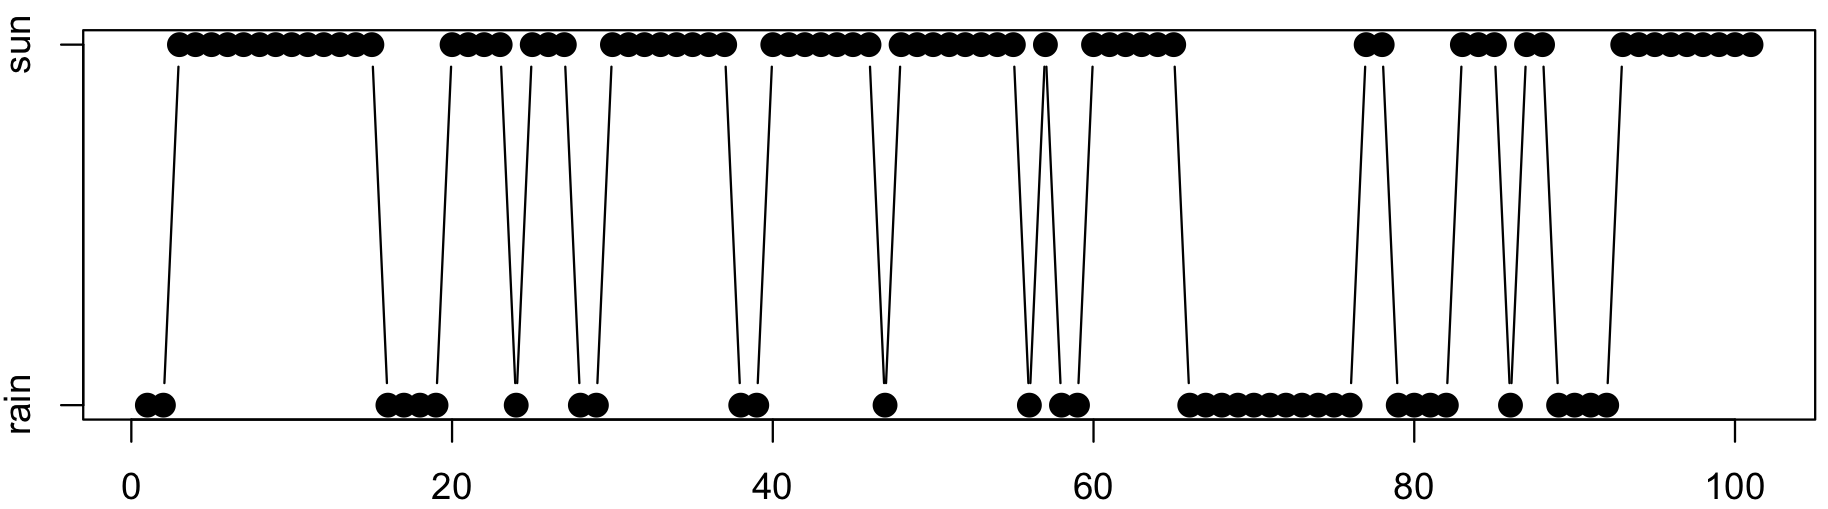
\includegraphics[width=0.7\linewidth]{img/markov_chain_example_analysis}
\end{center}
The forecast of the weather in the distant future is nearly independent from the current state.

\begin{theorem}
	A Markov chain $\{X_t ,t \in \mathbb{N}\}$ is a sequence of random variables $X_t$ in discrete time $t \in \mathbb{N}$ on a state space $S$, that randomly visits one state after another. At each step the random movement to the next state depends only on the previous state.
	
	$$ X_1 \rightarrow X_2 \rightarrow X_3 \rightarrow \dots \rightarrow X_{t-1} \rightarrow X_t \rightarrow \dots $$
	$$ P(X_t|X_{t-1},\cdots,X_1) = P(X_t|X_{t-1}) $$
	
	A Markov chain is given by a transition matrix or kernel $P_{x\rightarrow y} = P(y|x)$ for all $x,y \in S$ on a discrete or continous state space $S$.
\end{theorem}

Every \textbf{ergodic}, that is irreducible and aperiodic, Markov chain has a stationary distribution $\pi$. The \textbf{stationary distribution} is a probability distribution that remains unchanged under the transition probabilities of the chain as time progresses.

\begin{figure}[H]
	\begin{subfigure}[t]{0.45\linewidth}
		\centering
		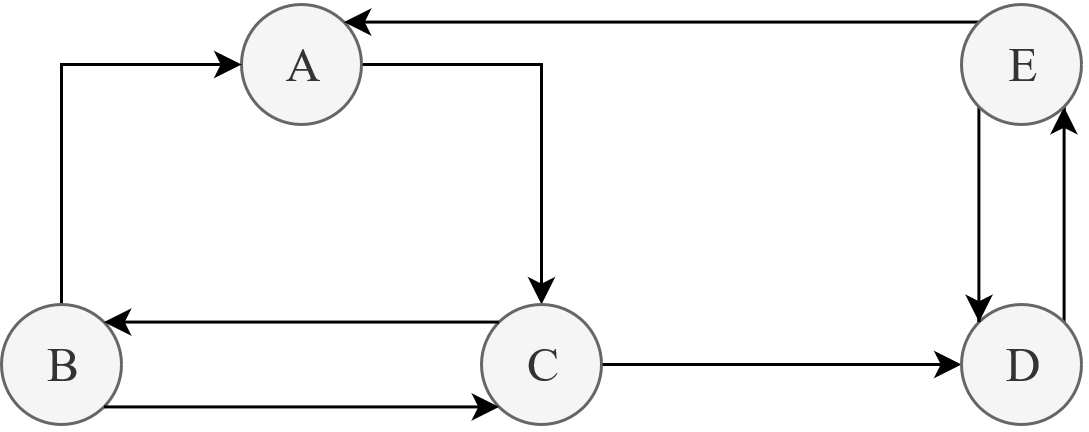
\includegraphics[width=\linewidth]{markov_chain_irreducibility}
		\caption{A Markov chain is \textbf{irreducible} iff there is a possible probability to get from any state to any other state}
	\end{subfigure}
	\hspace{0.1\linewidth}
	\begin{subfigure}[t]{0.45\linewidth}
		\centering
		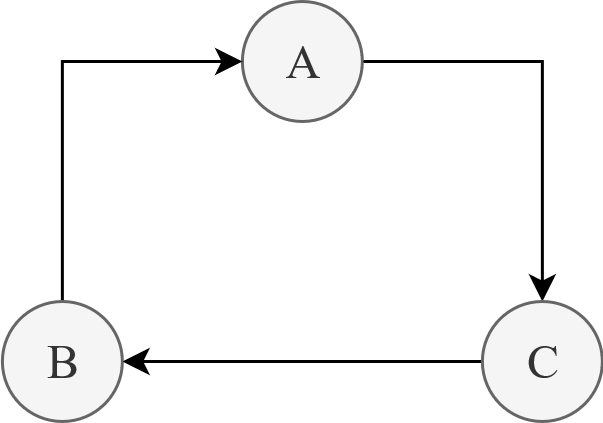
\includegraphics[width=0.6\linewidth]{markov_chain_periodicity}
		\caption{A Markov chain is \textbf{periodic} if you can visit certain states only at periodically recurring time steps.}
	\end{subfigure}
\end{figure}

The update for a Markov chain distribution can be formally expressed as
\begin{equation*}
	\forall x\in S: \pi(x) = \sum_{y\in S} \pi(y) P_{y\rightarrow x}
\end{equation*}

Consider an ergodic Markov chain $\{X_t ,t \in \mathbb{N}\}$ with stationary distribution $\pi$. Independent from the starting value $X_1$ the Markov chain converges to its stationary distribution $\pi$.
That means with increasing time $t$ the probability of being in state $x \in S$ reaches $\pi(x)$. If you run the Markov chain (infinitely) long, every state $x \in S$ is visited with fraction $\pi$(x).

If a distribution $\pi$ satisfies detailed balance, that is if
\begin{equation*}
	\pi(x)P_{x\rightarrow y} = \pi(y) P_{y\rightarrow x}
\end{equation*}

holds for all $x,y \in S$, then $\pi(x)$ does not change under the transition kernel and thus is a \textbf{stationary distribution}.

Markov Chain Monte Carlo denotes a class of algorithms for sampling from an arbitrary probability distribution. Construct a Markov chain that has the desired distribution as its stationary distribution to sample from the desired distribution.

\begin{itemize}
	\item Run the chain with an arbitrary start value
	\item Discard the first steps (burn-in), until the assumption that the chain is independent from its start value is satisfied
	\item Now pick values from the chain at certain periods of steps to get an i.i.d. sample from the stationary distribution
\end{itemize}

\subsection{Metropolis Hastings}

Let $\pi(\theta)$ be a probability density, for example the posterior $P(\theta|D)$. The Metropolis Hastings algorithm constructs a Markov chain on the parameter space, such that the density $\pi(\theta)$ is the equilibrium distribution.

Let $Q(\theta_{prop} |\theta)$ be a proposal distribution, that generates a new set of parameters $\theta_{prop}$ given the current set of parameters $\theta$. Often this is done by slightly changing $\theta$.

Iterate:
\begin{enumerate}
	\item Proposal: Simulate $\theta_{prop} \sim Q(\theta_{prop} |\theta)$
	\item Acceptance: Simulate $u \sim Unif(0,1)$\\
	$$\text{If }\frac{\pi(\theta_{prop})Q(\theta|\theta_{prop} )}{\pi(\theta) Q(\theta_{prop} |\theta)}> u\text{ set }\theta = \theta_{prop}$$
\end{enumerate}

\subsubsection{Remarks on the Metropolis Hastings Algorithm}
The desired probability density $\pi(\theta)$ only needs to be known up to a multiplicative constant, because factors cancel out in Metropolis Hastings ratio:$\frac{\pi(\theta_{prop})Q(\theta|\theta_{prop} )}{\pi(\theta) Q(\theta_{prop} |\theta)}$. So its sufficient to know the unnormalized probability density.

The quality of the MH algorithm depends on a good proposal distribution $Q(\theta|\theta_{prop})$: If $Q(\theta|\theta_{prop})$ proposes states in a too close neighbourhood, nearly every state is accepted, but the chain is moving very slow and samples are highly correlated. If $Q(\theta|\theta_{prop})$ proposes states in a too broad neighbourhood, too many states are rejected.

\subsubsection{Metropolis Rejection}
If $\pi(\theta)$ is a probability density on the parameter space $\mathbb{R}^d$, choose $z \sim Q$ to be a $d$-dimensional, mean-zero, multivariate normal distributed random variable and set $\theta_{prop} = \theta + z$.

Then the proposal density is symmetric and therefore: $Q(\theta|\theta_{prop} ) = Q(\theta_{prop} |\theta)$.

Iterate:
\begin{enumerate}
	\item Proposal: Simulate $z \sim Q$ and set $\theta_{prop} = \theta + z$
	\item Metropolis Rejection: Simulate $u \sim Unif(0,1)$\\
	$$\text{If }\frac{\pi(\theta_{prop})}{\pi(\theta)}> u\text{ set }\theta = \theta_{prop}$$
\end{enumerate}

\subsubsection{Monte Carlo Markov Chain Diagnostics}

\begin{itemize}
	\item How to choose a good proposal distribution?
	\item Proposal distributions: Adjust smaller / higher variance
	\item Scatterplot of data
	\item Trace plot should look like a caterpillar
	\item Discard burn-in
\end{itemize}

% ------------------------ APPENDIX ------------------------
\clearpage
\newpage
\appendix
\section{Exercises}

\subsection{Exercise 01}
\inputminted[linenos,breaklines,fontsize=\small]{R}{RCode/01_Exercise01.R}

\subsection{Exercise 02}
\inputminted[linenos,breaklines,fontsize=\small]{R}{RCode/02_Exercise02.R}

\subsection{Exercise 03}
\inputminted[linenos,breaklines,fontsize=\small]{R}{RCode/03_Exercise03.R}

\subsection{Exercise 04}
\inputminted[linenos,breaklines,fontsize=\small]{R}{RCode/04_Exercise04.R}

\subsection{Exercise 05}
\inputminted[linenos,breaklines,fontsize=\small]{R}{RCode/05_Exercise05.R}

\subsection{Exercise 06}
\inputminted[linenos,breaklines,fontsize=\small]{R}{RCode/06_Exercise06.R}

\subsection{Exercise 08}
\inputminted[linenos,breaklines,fontsize=\small]{R}{RCode/07_Exercise08.R}

\subsection{Exercise 09}
\inputminted[linenos,breaklines,fontsize=\small]{R}{RCode/09_Exercise09.R}

\subsection{Exercise 10}
\inputminted[linenos,breaklines,fontsize=\small]{R}{RCode/10_Exercise10.R}

\subsection{Exercise 11}
\inputminted[linenos,breaklines,fontsize=\small]{R}{RCode/11_Exercise11.R}

\subsection{Exercise 12}
\inputminted[linenos,breaklines,fontsize=\small]{R}{RCode/12_Exercise12.R}

\subsection{Exercise 13}
\inputminted[linenos,breaklines,fontsize=\small]{R}{RCode/13_Exercise13.R}

\subsection{Exercise 14}
\inputminted[linenos,breaklines,fontsize=\small]{R}{RCode/14_Exercise14.R}


\end{document}
